\documentclass[1p]{elsarticle_modified}
%\bibliographystyle{elsarticle-num}

%\usepackage[colorlinks]{hyperref}
%\usepackage{abbrmath_seonhwa} %\Abb, \Ascr, \Acal ,\Abf, \Afrak
\usepackage{amsfonts}
\usepackage{amssymb}
\usepackage{amsmath}
\usepackage{amsthm}
\usepackage{scalefnt}
\usepackage{amsbsy}
\usepackage{kotex}
\usepackage{caption}
\usepackage{subfig}
\usepackage{color}
\usepackage{graphicx}
\usepackage{xcolor} %% white, black, red, green, blue, cyan, magenta, yellow
\usepackage{float}
\usepackage{setspace}
\usepackage{hyperref}

\usepackage{tikz}
\usetikzlibrary{arrows}

\usepackage{multirow}
\usepackage{array} % fixed length table
\usepackage{hhline}

%%%%%%%%%%%%%%%%%%%%%
\makeatletter
\renewcommand*\env@matrix[1][\arraystretch]{%
	\edef\arraystretch{#1}%
	\hskip -\arraycolsep
	\let\@ifnextchar\new@ifnextchar
	\array{*\c@MaxMatrixCols c}}
\makeatother %https://tex.stackexchange.com/questions/14071/how-can-i-increase-the-line-spacing-in-a-matrix
%%%%%%%%%%%%%%%

\usepackage[normalem]{ulem}

\newcommand{\msout}[1]{\ifmmode\text{\sout{\ensuremath{#1}}}\else\sout{#1}\fi}
%SOURCE: \msout is \stkout macro in https://tex.stackexchange.com/questions/20609/strikeout-in-math-mode

\newcommand{\cancel}[1]{
	\ifmmode
	{\color{red}\msout{#1}}
	\else
	{\color{red}\sout{#1}}
	\fi
}

\newcommand{\add}[1]{
	{\color{blue}\uwave{#1}}
}

\newcommand{\replace}[2]{
	\ifmmode
	{\color{red}\msout{#1}}{\color{blue}\uwave{#2}}
	\else
	{\color{red}\sout{#1}}{\color{blue}\uwave{#2}}
	\fi
}

\newcommand{\Sol}{\mathcal{S}} %segment
\newcommand{\D}{D} %diagram
\newcommand{\A}{\mathcal{A}} %arc


%%%%%%%%%%%%%%%%%%%%%%%%%%%%%5 test

\def\sl{\operatorname{\textup{SL}}(2,\Cbb)}
\def\psl{\operatorname{\textup{PSL}}(2,\Cbb)}
\def\quan{\mkern 1mu \triangleright \mkern 1mu}

\theoremstyle{definition}
\newtheorem{thm}{Theorem}[section]
\newtheorem{prop}[thm]{Proposition}
\newtheorem{lem}[thm]{Lemma}
\newtheorem{ques}[thm]{Question}
\newtheorem{cor}[thm]{Corollary}
\newtheorem{defn}[thm]{Definition}
\newtheorem{exam}[thm]{Example}
\newtheorem{rmk}[thm]{Remark}
\newtheorem{alg}[thm]{Algorithm}

\newcommand{\I}{\sqrt{-1}}
\begin{document}

%\begin{frontmatter}
%
%\title{Boundary parabolic representations of knots up to 8 crossings}
%
%%% Group authors per affiliation:
%\author{Yunhi Cho} 
%\address{Department of Mathematics, University of Seoul, Seoul, Korea}
%\ead{yhcho@uos.ac.kr}
%
%
%\author{Seonhwa Kim} %\fnref{s_kim}}
%\address{Center for Geometry and Physics, Institute for Basic Science, Pohang, 37673, Korea}
%\ead{ryeona17@ibs.re.kr}
%
%\author{Hyuk Kim}
%\address{Department of Mathematical Sciences, Seoul National University, Seoul 08826, Korea}
%\ead{hyukkim@snu.ac.kr}
%
%\author{Seokbeom Yoon}
%\address{Department of Mathematical Sciences, Seoul National University, Seoul, 08826,  Korea}
%\ead{sbyoon15@snu.ac.kr}
%
%\begin{abstract}
%We find all boundary parabolic representation of knots up to 8 crossings.
%
%\end{abstract}
%\begin{keyword}
%    \MSC[2010] 57M25 
%\end{keyword}
%
%\end{frontmatter}

%\linenumbers
%\tableofcontents
%
\newcommand\colored[1]{\textcolor{white}{\rule[-0.35ex]{0.8em}{1.4ex}}\kern-0.8em\color{red} #1}%
%\newcommand\colored[1]{\textcolor{white}{ #1}\kern-2.17ex	\textcolor{white}{ #1}\kern-1.81ex	\textcolor{white}{ #1}\kern-2.15ex\color{red}#1	}

{\Large $\underline{12a_{0960}~(K12a_{0960})}$}

\setlength{\tabcolsep}{10pt}
\renewcommand{\arraystretch}{1.6}
\vspace{1cm}\begin{tabular}{m{100pt}>{\centering\arraybackslash}m{274pt}}
\multirow{5}{120pt}{
	\centering
	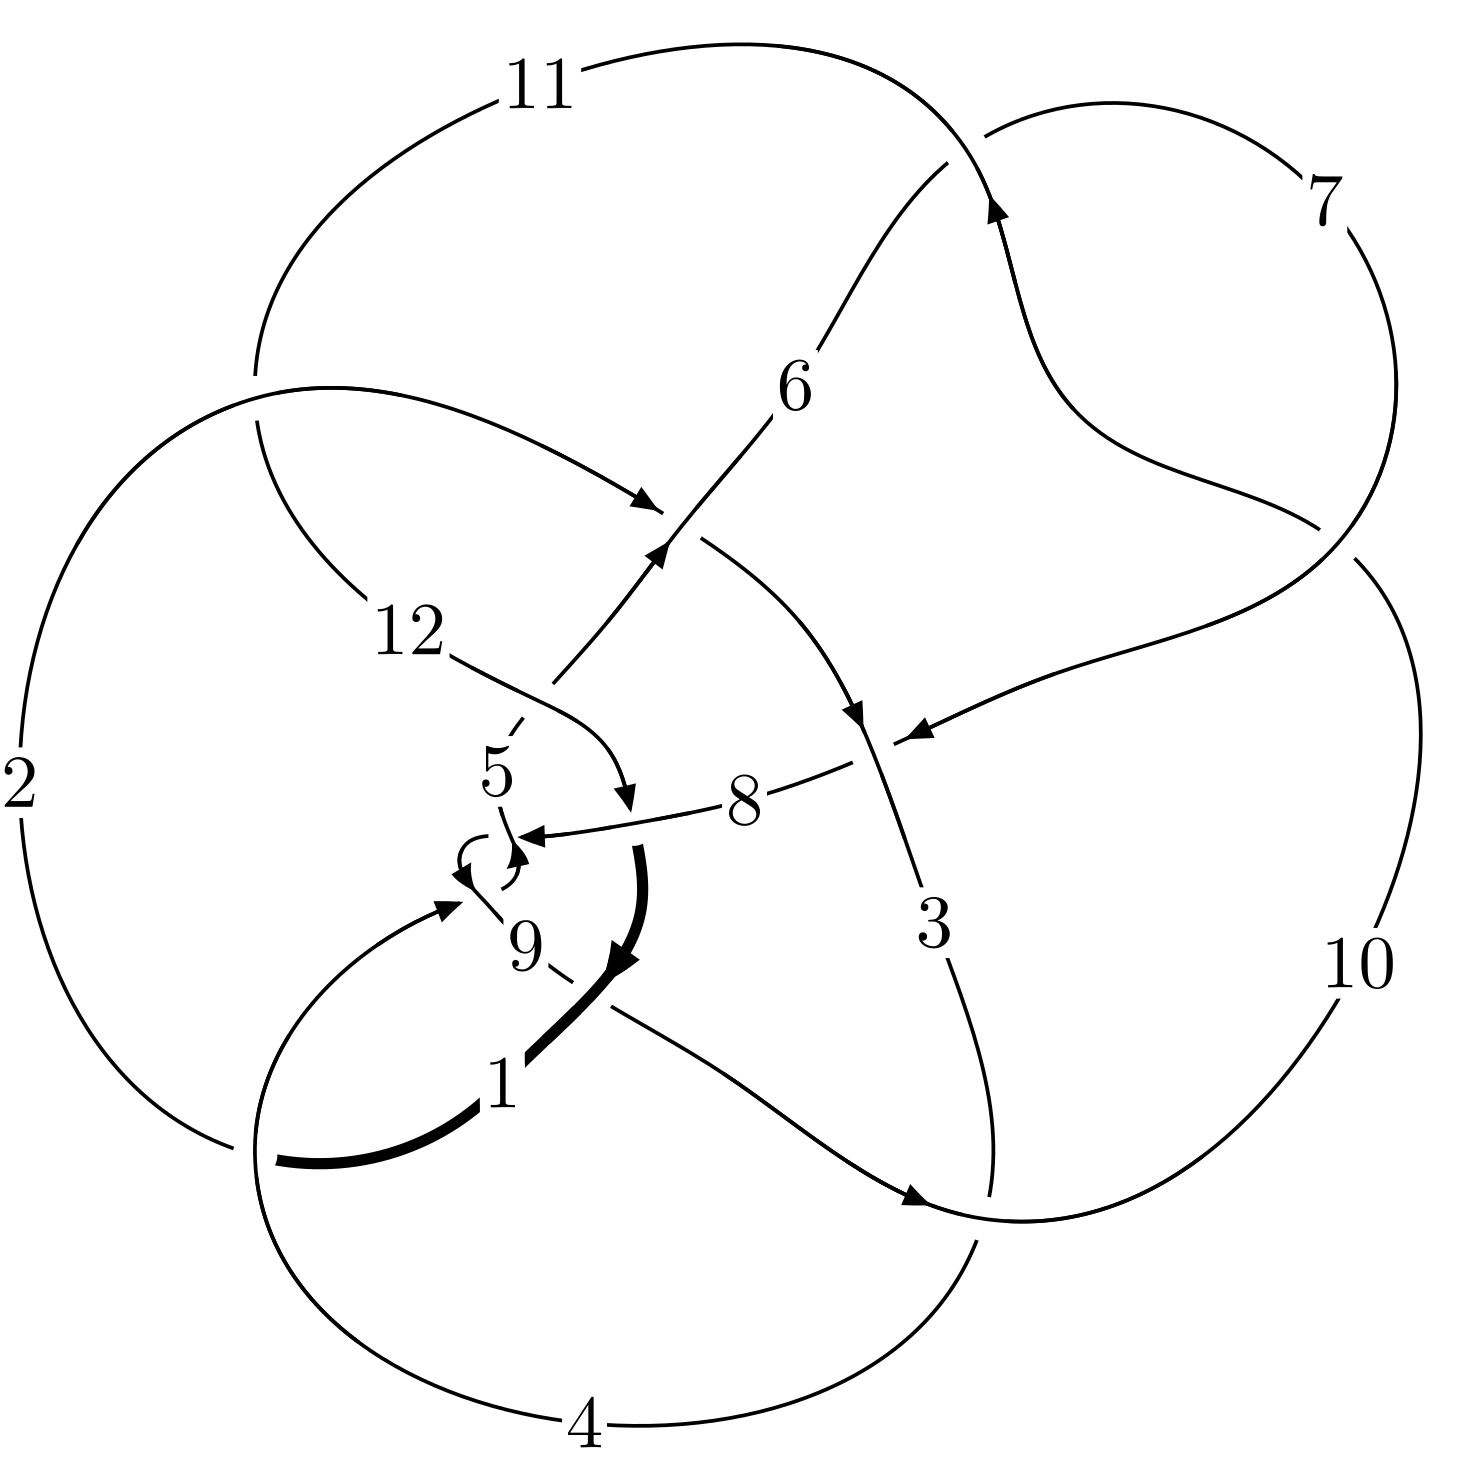
\includegraphics[width=112pt]{../../../GIT/diagram.site/Diagrams/png/1761_12a_0960.png}\\
\ \ \ A knot diagram\footnotemark}&
\allowdisplaybreaks
\textbf{Linearized knot diagam} \\
\cline{2-2}
 &
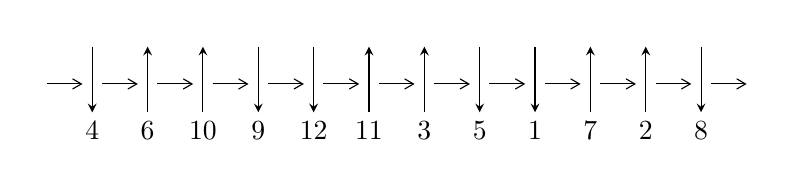
\begin{tikzpicture}[x=20pt, y=17pt]
	% nodes
	\node (C0) at (0, 0) {};
	\node (C1) at (1, 0) {};
	\node (C1U) at (1, +1) {};
	\node (C1D) at (1, -1) {4};

	\node (C2) at (2, 0) {};
	\node (C2U) at (2, +1) {};
	\node (C2D) at (2, -1) {6};

	\node (C3) at (3, 0) {};
	\node (C3U) at (3, +1) {};
	\node (C3D) at (3, -1) {10};

	\node (C4) at (4, 0) {};
	\node (C4U) at (4, +1) {};
	\node (C4D) at (4, -1) {9};

	\node (C5) at (5, 0) {};
	\node (C5U) at (5, +1) {};
	\node (C5D) at (5, -1) {12};

	\node (C6) at (6, 0) {};
	\node (C6U) at (6, +1) {};
	\node (C6D) at (6, -1) {11};

	\node (C7) at (7, 0) {};
	\node (C7U) at (7, +1) {};
	\node (C7D) at (7, -1) {3};

	\node (C8) at (8, 0) {};
	\node (C8U) at (8, +1) {};
	\node (C8D) at (8, -1) {5};

	\node (C9) at (9, 0) {};
	\node (C9U) at (9, +1) {};
	\node (C9D) at (9, -1) {1};

	\node (C10) at (10, 0) {};
	\node (C10U) at (10, +1) {};
	\node (C10D) at (10, -1) {7};

	\node (C11) at (11, 0) {};
	\node (C11U) at (11, +1) {};
	\node (C11D) at (11, -1) {2};

	\node (C12) at (12, 0) {};
	\node (C12U) at (12, +1) {};
	\node (C12D) at (12, -1) {8};
	\node (C13) at (13, 0) {};

	% arrows
	\draw[->,>={angle 60}]
	(C0) edge (C1) (C1) edge (C2) (C2) edge (C3) (C3) edge (C4) (C4) edge (C5) (C5) edge (C6) (C6) edge (C7) (C7) edge (C8) (C8) edge (C9) (C9) edge (C10) (C10) edge (C11) (C11) edge (C12) (C12) edge (C13) ;	\draw[->,>=stealth]
	(C1U) edge (C1D) (C2D) edge (C2U) (C3D) edge (C3U) (C4U) edge (C4D) (C5U) edge (C5D) (C6D) edge (C6U) (C7D) edge (C7U) (C8U) edge (C8D) (C9U) edge (C9D) (C10D) edge (C10U) (C11D) edge (C11U) (C12U) edge (C12D) ;
	\end{tikzpicture} \\
\hhline{~~} \\& 
\textbf{Solving Sequence} \\ \cline{2-2} 
 &
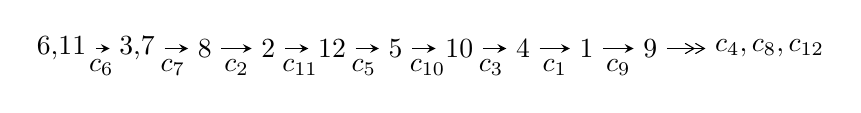
\begin{tikzpicture}[x=23pt, y=7pt]
	% node
	\node (A0) at (-1/8, 0) {6,11};
	\node (A1) at (17/16, 0) {3,7};
	\node (A2) at (17/8, 0) {8};
	\node (A3) at (25/8, 0) {2};
	\node (A4) at (33/8, 0) {12};
	\node (A5) at (41/8, 0) {5};
	\node (A6) at (49/8, 0) {10};
	\node (A7) at (57/8, 0) {4};
	\node (A8) at (65/8, 0) {1};
	\node (A9) at (73/8, 0) {9};
	\node (C1) at (1/2, -1) {$c_{6}$};
	\node (C2) at (13/8, -1) {$c_{7}$};
	\node (C3) at (21/8, -1) {$c_{2}$};
	\node (C4) at (29/8, -1) {$c_{11}$};
	\node (C5) at (37/8, -1) {$c_{5}$};
	\node (C6) at (45/8, -1) {$c_{10}$};
	\node (C7) at (53/8, -1) {$c_{3}$};
	\node (C8) at (61/8, -1) {$c_{1}$};
	\node (C9) at (69/8, -1) {$c_{9}$};
	\node (A10) at (11, 0) {$c_{4},c_{8},c_{12}$};

	% edge
	\draw[->,>=stealth]	
	(A0) edge (A1) (A1) edge (A2) (A2) edge (A3) (A3) edge (A4) (A4) edge (A5) (A5) edge (A6) (A6) edge (A7) (A7) edge (A8) (A8) edge (A9) ;
	\draw[->>,>={angle 60}]	
	(A9) edge (A10);
\end{tikzpicture} \\ 

\end{tabular} \\

\footnotetext{
The image of knot diagram is generated by the software ``\textbf{Draw programme}" developed by Andrew Bartholomew(\url{http://www.layer8.co.uk/maths/draw/index.htm\#Running-draw}), where we modified some parts for our purpose(\url{https://github.com/CATsTAILs/LinksPainter}).
}\phantom \\ \newline 
\centering \textbf{Ideals for irreducible components\footnotemark of $X_{\text{par}}$} 
 
\begin{align*}
I^u_{1}&=\langle 
6.32511\times10^{1035} u^{175}+4.24899\times10^{1036} u^{174}+\cdots+4.69972\times10^{1036} b+3.27998\times10^{1038},\\
\phantom{I^u_{1}}&\phantom{= \langle  }8.00347\times10^{1038} u^{175}+5.25942\times10^{1039} u^{174}+\cdots+4.41303\times10^{1039} a+3.29768\times10^{1041},\\
\phantom{I^u_{1}}&\phantom{= \langle  }u^{176}+6 u^{175}+\cdots-5650 u+939\rangle \\
I^u_{2}&=\langle 
-1.39268\times10^{28} u^{33}+3.61198\times10^{28} u^{32}+\cdots+5.54335\times10^{28} b+8.01444\times10^{28},\\
\phantom{I^u_{2}}&\phantom{= \langle  }-1.75682\times10^{28} u^{33}+3.90770\times10^{28} u^{32}+\cdots+5.54335\times10^{28} a-1.15604\times10^{29},\\
\phantom{I^u_{2}}&\phantom{= \langle  }u^{34}+16 u^{32}+\cdots-15 u+1\rangle \\
I^u_{3}&=\langle 
b+u,\;a+u+1,\;u^2+u+1\rangle \\
\\
\end{align*}
\raggedright * 3 irreducible components of $\dim_{\mathbb{C}}=0$, with total 212 representations.\\
\footnotetext{All coefficients of polynomials are rational numbers. But the coefficients are sometimes approximated in decimal forms when there is not enough margin.}
\newpage
\renewcommand{\arraystretch}{1}
\centering \section*{I. $I^u_{1}= \langle 6.33\times10^{1035} u^{175}+4.25\times10^{1036} u^{174}+\cdots+4.70\times10^{1036} b+3.28\times10^{1038},\;8.00\times10^{1038} u^{175}+5.26\times10^{1039} u^{174}+\cdots+4.41\times10^{1039} a+3.30\times10^{1041},\;u^{176}+6 u^{175}+\cdots-5650 u+939 \rangle$}
\flushleft \textbf{(i) Arc colorings}\\
\begin{tabular}{m{7pt} m{180pt} m{7pt} m{180pt} }
\flushright $a_{6}=$&$\begin{pmatrix}1\\0\end{pmatrix}$ \\
\flushright $a_{11}=$&$\begin{pmatrix}0\\u\end{pmatrix}$ \\
\flushright $a_{3}=$&$\begin{pmatrix}-0.181360 u^{175}-1.19179 u^{174}+\cdots+305.464 u-74.7260\\-0.134585 u^{175}-0.904096 u^{174}+\cdots+323.722 u-69.7909\end{pmatrix}$ \\
\flushright $a_{7}=$&$\begin{pmatrix}1\\- u^2\end{pmatrix}$ \\
\flushright $a_{8}=$&$\begin{pmatrix}-0.00219584 u^{175}-0.100916 u^{174}+\cdots+398.465 u-64.6077\\0.0390647 u^{175}+0.184706 u^{174}+\cdots+246.044 u-35.5061\end{pmatrix}$ \\
\flushright $a_{2}=$&$\begin{pmatrix}-0.0467749 u^{175}-0.287698 u^{174}+\cdots-18.2581 u-4.93505\\-0.134585 u^{175}-0.904096 u^{174}+\cdots+323.722 u-69.7909\end{pmatrix}$ \\
\flushright $a_{12}=$&$\begin{pmatrix}0.00720057 u^{175}+0.0727156 u^{174}+\cdots-80.4218 u+10.4860\\-0.171963 u^{175}-0.989112 u^{174}+\cdots-298.311 u+29.0343\end{pmatrix}$ \\
\flushright $a_{5}=$&$\begin{pmatrix}0.111561 u^{175}+0.549967 u^{174}+\cdots+607.097 u-85.9822\\-0.319703 u^{175}-1.89062 u^{174}+\cdots-365.057 u+23.6912\end{pmatrix}$ \\
\flushright $a_{10}=$&$\begin{pmatrix}- u\\u^3+u\end{pmatrix}$ \\
\flushright $a_{4}=$&$\begin{pmatrix}-0.0710434 u^{175}-0.435873 u^{174}+\cdots-20.1901 u-7.61312\\-0.0970434 u^{175}-0.650749 u^{174}+\cdots+221.741 u-48.6175\end{pmatrix}$ \\
\flushright $a_{1}=$&$\begin{pmatrix}0.0186189 u^{175}+0.0662415 u^{174}+\cdots+232.284 u-37.5107\\-0.112061 u^{175}-0.612880 u^{174}+\cdots-344.134 u+45.3503\end{pmatrix}$ \\
\flushright $a_{9}=$&$\begin{pmatrix}0.0861891 u^{175}+0.595903 u^{174}+\cdots-265.966 u+55.0977\\0.0391470 u^{175}-0.195411 u^{174}+\cdots+1864.59 u-304.617\end{pmatrix}$\\&\end{tabular}
\flushleft \textbf{(ii) Obstruction class $= -1$}\\~\\
\flushleft \textbf{(iii) Cusp Shapes $= 1.92136 u^{175}+12.8967 u^{174}+\cdots-4562.99 u+988.525$}\\~\\
\newpage\renewcommand{\arraystretch}{1}
\flushleft \textbf{(iv) u-Polynomials at the component}\newline \\
\begin{tabular}{m{50pt}|m{274pt}}
Crossings & \hspace{64pt}u-Polynomials at each crossing \\
\hline $$\begin{aligned}c_{1}\end{aligned}$$&$\begin{aligned}
&u^{176}+7 u^{175}+\cdots+69156 u+17323
\end{aligned}$\\
\hline $$\begin{aligned}c_{2}\end{aligned}$$&$\begin{aligned}
&4(4 u^{176}-42 u^{175}+\cdots+4 u+3)
\end{aligned}$\\
\hline $$\begin{aligned}c_{3}\end{aligned}$$&$\begin{aligned}
&4(4 u^{176}+18 u^{175}+\cdots+1.69296\times10^{9} u+1.02369\times10^{8})
\end{aligned}$\\
\hline $$\begin{aligned}c_{4},c_{8}\end{aligned}$$&$\begin{aligned}
&u^{176}+6 u^{175}+\cdots-5650 u+939
\end{aligned}$\\
\hline $$\begin{aligned}c_{5}\end{aligned}$$&$\begin{aligned}
&4(4 u^{176}-18 u^{175}+\cdots-1.69296\times10^{9} u+1.02369\times10^{8})
\end{aligned}$\\
\hline $$\begin{aligned}c_{6},c_{10}\end{aligned}$$&$\begin{aligned}
&u^{176}-6 u^{175}+\cdots+5650 u+939
\end{aligned}$\\
\hline $$\begin{aligned}c_{7}\end{aligned}$$&$\begin{aligned}
&u^{176}+u^{175}+\cdots-12001832 u+1637744
\end{aligned}$\\
\hline $$\begin{aligned}c_{9}\end{aligned}$$&$\begin{aligned}
&4(4 u^{176}+42 u^{175}+\cdots-4 u+3)
\end{aligned}$\\
\hline $$\begin{aligned}c_{11}\end{aligned}$$&$\begin{aligned}
&u^{176}-7 u^{175}+\cdots-69156 u+17323
\end{aligned}$\\
\hline $$\begin{aligned}c_{12}\end{aligned}$$&$\begin{aligned}
&u^{176}- u^{175}+\cdots+12001832 u+1637744
\end{aligned}$\\
\hline
\end{tabular}\\~\\
\newpage\renewcommand{\arraystretch}{1}
\flushleft \textbf{(v) Riley Polynomials at the component}\newline \\
\begin{tabular}{m{50pt}|m{274pt}}
Crossings & \hspace{64pt}Riley Polynomials at each crossing \\
\hline $$\begin{aligned}c_{1},c_{11}\end{aligned}$$&$\begin{aligned}
&y^{176}+11 y^{175}+\cdots+18368043448 y+300086329
\end{aligned}$\\
\hline $$\begin{aligned}c_{2},c_{9}\end{aligned}$$&$\begin{aligned}
&16(16 y^{176}+164 y^{175}+\cdots+632 y+9)
\end{aligned}$\\
\hline $$\begin{aligned}c_{3},c_{5}\end{aligned}$$&$\begin{aligned}
&16(16 y^{176}+1348 y^{175}+\cdots+6.24455\times10^{17} y+1.04794\times10^{16})
\end{aligned}$\\
\hline $$\begin{aligned}c_{4},c_{6},c_{8}\\c_{10}\end{aligned}$$&$\begin{aligned}
&y^{176}+134 y^{175}+\cdots+23450330 y+881721
\end{aligned}$\\
\hline $$\begin{aligned}c_{7},c_{12}\end{aligned}$$&$\begin{aligned}
&y^{176}+51 y^{175}+\cdots+119113228533312 y+2682205409536
\end{aligned}$\\
\hline
\end{tabular}\\~\\
\newpage\flushleft \textbf{(vi) Complex Volumes and Cusp Shapes}
$$\begin{array}{c|c|c}  
\text{Solutions to }I^u_{1}& \I (\text{vol} + \sqrt{-1}CS) & \text{Cusp shape}\\
 \hline 
\begin{aligned}
u &= -0.268225 + 0.962582 I \\
a &= \phantom{-}0.20659 + 2.76799 I \\
b &= -0.264729 + 0.026201 I\end{aligned}
 & \phantom{-}2.66927 - 10.63920 I & \phantom{-0.000000 } 0 \\ \hline\begin{aligned}
u &= -0.268225 - 0.962582 I \\
a &= \phantom{-}0.20659 - 2.76799 I \\
b &= -0.264729 - 0.026201 I\end{aligned}
 & \phantom{-}2.66927 + 10.63920 I & \phantom{-0.000000 } 0 \\ \hline\begin{aligned}
u &= -0.639498 + 0.779579 I \\
a &= -0.914982 - 0.304342 I \\
b &= \phantom{-}0.645237 - 0.266582 I\end{aligned}
 & \phantom{-}0.73655 - 2.57695 I & \phantom{-0.000000 } 0 \\ \hline\begin{aligned}
u &= -0.639498 - 0.779579 I \\
a &= -0.914982 + 0.304342 I \\
b &= \phantom{-}0.645237 + 0.266582 I\end{aligned}
 & \phantom{-}0.73655 + 2.57695 I & \phantom{-0.000000 } 0 \\ \hline\begin{aligned}
u &= -0.403534 + 0.894931 I \\
a &= -0.490359 - 1.134190 I \\
b &= \phantom{-}0.150323 - 0.171101 I\end{aligned}
 & \phantom{-}0.36799 - 1.98151 I & \phantom{-0.000000 } 0 \\ \hline\begin{aligned}
u &= -0.403534 - 0.894931 I \\
a &= -0.490359 + 1.134190 I \\
b &= \phantom{-}0.150323 + 0.171101 I\end{aligned}
 & \phantom{-}0.36799 + 1.98151 I & \phantom{-0.000000 } 0 \\ \hline\begin{aligned}
u &= \phantom{-}0.024715 + 0.972378 I \\
a &= -1.005110 - 0.313765 I \\
b &= \phantom{-}1.063340 - 0.252710 I\end{aligned}
 & \phantom{-}4.15953 - 4.46103 I & \phantom{-0.000000 } 0 \\ \hline\begin{aligned}
u &= \phantom{-}0.024715 - 0.972378 I \\
a &= -1.005110 + 0.313765 I \\
b &= \phantom{-}1.063340 + 0.252710 I\end{aligned}
 & \phantom{-}4.15953 + 4.46103 I & \phantom{-0.000000 } 0 \\ \hline\begin{aligned}
u &= -0.098010 + 1.027020 I \\
a &= -1.36993 - 1.20050 I \\
b &= -1.62456 - 0.79093 I\end{aligned}
 & \phantom{-}0.714090 - 0.355524 I & \phantom{-0.000000 } 0 \\ \hline\begin{aligned}
u &= -0.098010 - 1.027020 I \\
a &= -1.36993 + 1.20050 I \\
b &= -1.62456 + 0.79093 I\end{aligned}
 & \phantom{-}0.714090 + 0.355524 I & \phantom{-0.000000 } 0\\
 \hline 
 \end{array}$$\newpage$$\begin{array}{c|c|c}  
\text{Solutions to }I^u_{1}& \I (\text{vol} + \sqrt{-1}CS) & \text{Cusp shape}\\
 \hline 
\begin{aligned}
u &= \phantom{-}0.644866 + 0.808232 I \\
a &= \phantom{-}0.648376 - 0.508937 I \\
b &= -0.917957 - 0.040537 I\end{aligned}
 & \phantom{-}5.16399 + 2.60014 I & \phantom{-0.000000 } 0 \\ \hline\begin{aligned}
u &= \phantom{-}0.644866 - 0.808232 I \\
a &= \phantom{-}0.648376 + 0.508937 I \\
b &= -0.917957 + 0.040537 I\end{aligned}
 & \phantom{-}5.16399 - 2.60014 I & \phantom{-0.000000 } 0 \\ \hline\begin{aligned}
u &= \phantom{-}0.445760 + 0.834063 I \\
a &= \phantom{-}0.33232 - 1.43020 I \\
b &= -0.592928 - 0.020233 I\end{aligned}
 & \phantom{-}4.91221 + 2.00569 I & \phantom{-0.000000 } 0 \\ \hline\begin{aligned}
u &= \phantom{-}0.445760 - 0.834063 I \\
a &= \phantom{-}0.33232 + 1.43020 I \\
b &= -0.592928 + 0.020233 I\end{aligned}
 & \phantom{-}4.91221 - 2.00569 I & \phantom{-0.000000 } 0 \\ \hline\begin{aligned}
u &= -1.035470 + 0.205784 I \\
a &= -0.078531 - 0.548387 I \\
b &= \phantom{-}0.803386 + 0.258956 I\end{aligned}
 & \phantom{-}5.06643 + 0.78586 I & \phantom{-0.000000 } 0 \\ \hline\begin{aligned}
u &= -1.035470 - 0.205784 I \\
a &= -0.078531 + 0.548387 I \\
b &= \phantom{-}0.803386 - 0.258956 I\end{aligned}
 & \phantom{-}5.06643 - 0.78586 I & \phantom{-0.000000 } 0 \\ \hline\begin{aligned}
u &= -0.376648 + 0.863700 I \\
a &= -1.31412 - 0.99638 I \\
b &= -0.776206 - 0.933078 I\end{aligned}
 & \phantom{-}0.557762 - 0.871550 I & \phantom{-0.000000 } 0 \\ \hline\begin{aligned}
u &= -0.376648 - 0.863700 I \\
a &= -1.31412 + 0.99638 I \\
b &= -0.776206 + 0.933078 I\end{aligned}
 & \phantom{-}0.557762 + 0.871550 I & \phantom{-0.000000 } 0 \\ \hline\begin{aligned}
u &= -0.783561 + 0.519734 I \\
a &= -0.283303 - 0.093269 I \\
b &= \phantom{-}1.072940 - 0.564679 I\end{aligned}
 & \phantom{-}3.57396 - 6.11171 I & \phantom{-0.000000 } 0 \\ \hline\begin{aligned}
u &= -0.783561 - 0.519734 I \\
a &= -0.283303 + 0.093269 I \\
b &= \phantom{-}1.072940 + 0.564679 I\end{aligned}
 & \phantom{-}3.57396 + 6.11171 I & \phantom{-0.000000 } 0\\
 \hline 
 \end{array}$$\newpage$$\begin{array}{c|c|c}  
\text{Solutions to }I^u_{1}& \I (\text{vol} + \sqrt{-1}CS) & \text{Cusp shape}\\
 \hline 
\begin{aligned}
u &= -1.060870 + 0.134806 I \\
a &= -0.091627 + 0.411572 I \\
b &= -0.939105 + 0.646913 I\end{aligned}
 & \phantom{-}3.81603 - 2.52639 I & \phantom{-0.000000 } 0 \\ \hline\begin{aligned}
u &= -1.060870 - 0.134806 I \\
a &= -0.091627 - 0.411572 I \\
b &= -0.939105 - 0.646913 I\end{aligned}
 & \phantom{-}3.81603 + 2.52639 I & \phantom{-0.000000 } 0 \\ \hline\begin{aligned}
u &= \phantom{-}0.267369 + 1.038610 I \\
a &= \phantom{-}0.13106 - 1.76673 I \\
b &= -0.93471 - 1.32000 I\end{aligned}
 & -1.21991 + 3.70716 I & \phantom{-0.000000 } 0 \\ \hline\begin{aligned}
u &= \phantom{-}0.267369 - 1.038610 I \\
a &= \phantom{-}0.13106 + 1.76673 I \\
b &= -0.93471 + 1.32000 I\end{aligned}
 & -1.21991 - 3.70716 I & \phantom{-0.000000 } 0 \\ \hline\begin{aligned}
u &= \phantom{-}0.064822 + 1.096500 I \\
a &= -0.123853 - 0.899928 I \\
b &= -1.44021 - 0.54781 I\end{aligned}
 & -1.86863 + 2.42778 I & \phantom{-0.000000 } 0 \\ \hline\begin{aligned}
u &= \phantom{-}0.064822 - 1.096500 I \\
a &= -0.123853 + 0.899928 I \\
b &= -1.44021 + 0.54781 I\end{aligned}
 & -1.86863 - 2.42778 I & \phantom{-0.000000 } 0 \\ \hline\begin{aligned}
u &= \phantom{-}0.934012 + 0.592825 I \\
a &= \phantom{-}0.733403 + 0.144804 I \\
b &= -0.694203 - 0.400242 I\end{aligned}
 & \phantom{-}3.48356 + 4.14986 I & \phantom{-0.000000 } 0 \\ \hline\begin{aligned}
u &= \phantom{-}0.934012 - 0.592825 I \\
a &= \phantom{-}0.733403 - 0.144804 I \\
b &= -0.694203 + 0.400242 I\end{aligned}
 & \phantom{-}3.48356 - 4.14986 I & \phantom{-0.000000 } 0 \\ \hline\begin{aligned}
u &= -0.879145 + 0.157980 I \\
a &= -0.391182 + 0.079087 I \\
b &= -0.965060 - 0.533810 I\end{aligned}
 & \phantom{-}2.95882 + 1.25298 I & \phantom{-0.000000 } 0 \\ \hline\begin{aligned}
u &= -0.879145 - 0.157980 I \\
a &= -0.391182 - 0.079087 I \\
b &= -0.965060 + 0.533810 I\end{aligned}
 & \phantom{-}2.95882 - 1.25298 I & \phantom{-0.000000 } 0\\
 \hline 
 \end{array}$$\newpage$$\begin{array}{c|c|c}  
\text{Solutions to }I^u_{1}& \I (\text{vol} + \sqrt{-1}CS) & \text{Cusp shape}\\
 \hline 
\begin{aligned}
u &= -0.026972 + 1.111890 I \\
a &= \phantom{-}0.25218 - 1.81916 I \\
b &= -0.913965 - 0.993863 I\end{aligned}
 & -2.35849 + 1.91634 I & \phantom{-0.000000 } 0 \\ \hline\begin{aligned}
u &= -0.026972 - 1.111890 I \\
a &= \phantom{-}0.25218 + 1.81916 I \\
b &= -0.913965 + 0.993863 I\end{aligned}
 & -2.35849 - 1.91634 I & \phantom{-0.000000 } 0 \\ \hline\begin{aligned}
u &= -0.101098 + 1.112320 I \\
a &= \phantom{-}0.747997 - 1.118490 I \\
b &= \phantom{-}1.92440 - 0.61397 I\end{aligned}
 & \phantom{-0.000000 } -3.38648 I & \phantom{-0.000000 } 0 \\ \hline\begin{aligned}
u &= -0.101098 - 1.112320 I \\
a &= \phantom{-}0.747997 + 1.118490 I \\
b &= \phantom{-}1.92440 + 0.61397 I\end{aligned}
 & \phantom{-0.000000 -}3.38648 I & \phantom{-0.000000 } 0 \\ \hline\begin{aligned}
u &= \phantom{-}0.830377 + 0.295226 I \\
a &= \phantom{-}0.534674 + 0.299283 I \\
b &= \phantom{-}0.997971 - 0.739870 I\end{aligned}
 & \phantom{-}7.09688 - 7.79945 I & \phantom{-0.000000 } 0 \\ \hline\begin{aligned}
u &= \phantom{-}0.830377 - 0.295226 I \\
a &= \phantom{-}0.534674 - 0.299283 I \\
b &= \phantom{-}0.997971 + 0.739870 I\end{aligned}
 & \phantom{-}7.09688 + 7.79945 I & \phantom{-0.000000 } 0 \\ \hline\begin{aligned}
u &= \phantom{-}0.677700 + 0.890752 I \\
a &= \phantom{-}0.315340 - 0.670034 I \\
b &= -0.069785 + 0.255534 I\end{aligned}
 & \phantom{-}2.35849 + 1.91634 I & \phantom{-0.000000 } 0 \\ \hline\begin{aligned}
u &= \phantom{-}0.677700 - 0.890752 I \\
a &= \phantom{-}0.315340 + 0.670034 I \\
b &= -0.069785 - 0.255534 I\end{aligned}
 & \phantom{-}2.35849 - 1.91634 I & \phantom{-0.000000 } 0 \\ \hline\begin{aligned}
u &= \phantom{-}0.023366 + 0.878538 I \\
a &= -0.844146 + 0.914953 I \\
b &= -0.042200 + 0.652552 I\end{aligned}
 & -1.21414 - 1.52821 I & \phantom{-0.000000 } 0 \\ \hline\begin{aligned}
u &= \phantom{-}0.023366 - 0.878538 I \\
a &= -0.844146 - 0.914953 I \\
b &= -0.042200 - 0.652552 I\end{aligned}
 & -1.21414 + 1.52821 I & \phantom{-0.000000 } 0\\
 \hline 
 \end{array}$$\newpage$$\begin{array}{c|c|c}  
\text{Solutions to }I^u_{1}& \I (\text{vol} + \sqrt{-1}CS) & \text{Cusp shape}\\
 \hline 
\begin{aligned}
u &= \phantom{-}0.470352 + 1.021550 I \\
a &= -0.817745 + 0.675912 I \\
b &= -0.352475 + 1.104280 I\end{aligned}
 & -0.557762 - 0.871550 I & \phantom{-0.000000 } 0 \\ \hline\begin{aligned}
u &= \phantom{-}0.470352 - 1.021550 I \\
a &= -0.817745 - 0.675912 I \\
b &= -0.352475 - 1.104280 I\end{aligned}
 & -0.557762 + 0.871550 I & \phantom{-0.000000 } 0 \\ \hline\begin{aligned}
u &= \phantom{-}0.114042 + 0.860315 I \\
a &= \phantom{-}1.72126 + 1.60013 I \\
b &= \phantom{-}0.335767 + 0.247262 I\end{aligned}
 & \phantom{-}4.26370 + 5.24171 I & \phantom{-0.000000 } 0 \\ \hline\begin{aligned}
u &= \phantom{-}0.114042 - 0.860315 I \\
a &= \phantom{-}1.72126 - 1.60013 I \\
b &= \phantom{-}0.335767 - 0.247262 I\end{aligned}
 & \phantom{-}4.26370 - 5.24171 I & \phantom{-0.000000 } 0 \\ \hline\begin{aligned}
u &= \phantom{-}1.124160 + 0.135421 I \\
a &= \phantom{-}0.0183299 + 0.1167330 I \\
b &= \phantom{-}0.897822 + 0.718916 I\end{aligned}
 & \phantom{-0.000000 -}9.56721 I & \phantom{-0.000000 } 0 \\ \hline\begin{aligned}
u &= \phantom{-}1.124160 - 0.135421 I \\
a &= \phantom{-}0.0183299 - 0.1167330 I \\
b &= \phantom{-}0.897822 - 0.718916 I\end{aligned}
 & \phantom{-0.000000 } -9.56721 I & \phantom{-0.000000 } 0 \\ \hline\begin{aligned}
u &= \phantom{-}1.134820 + 0.012898 I \\
a &= \phantom{-}0.145238 - 0.137047 I \\
b &= -0.800713 + 0.819560 I\end{aligned}
 & \phantom{-}4.74657 - 5.78864 I & \phantom{-0.000000 } 0 \\ \hline\begin{aligned}
u &= \phantom{-}1.134820 - 0.012898 I \\
a &= \phantom{-}0.145238 + 0.137047 I \\
b &= -0.800713 - 0.819560 I\end{aligned}
 & \phantom{-}4.74657 + 5.78864 I & \phantom{-0.000000 } 0 \\ \hline\begin{aligned}
u &= \phantom{-}0.211037 + 1.122750 I \\
a &= \phantom{-}0.78851 + 1.92789 I \\
b &= \phantom{-}0.059339 + 0.307011 I\end{aligned}
 & -3.57396 + 6.11171 I & \phantom{-0.000000 } 0 \\ \hline\begin{aligned}
u &= \phantom{-}0.211037 - 1.122750 I \\
a &= \phantom{-}0.78851 - 1.92789 I \\
b &= \phantom{-}0.059339 - 0.307011 I\end{aligned}
 & -3.57396 - 6.11171 I & \phantom{-0.000000 } 0\\
 \hline 
 \end{array}$$\newpage$$\begin{array}{c|c|c}  
\text{Solutions to }I^u_{1}& \I (\text{vol} + \sqrt{-1}CS) & \text{Cusp shape}\\
 \hline 
\begin{aligned}
u &= -0.001013 + 1.148490 I \\
a &= -0.98183 + 2.37273 I \\
b &= -1.50663 + 2.73217 I\end{aligned}
 & \phantom{-0.000000 -}1.35989 I & \phantom{-0.000000 } 0 \\ \hline\begin{aligned}
u &= -0.001013 - 1.148490 I \\
a &= -0.98183 - 2.37273 I \\
b &= -1.50663 - 2.73217 I\end{aligned}
 & \phantom{-0.000000 } -1.35989 I & \phantom{-0.000000 } 0 \\ \hline\begin{aligned}
u &= -0.808811 + 0.251963 I \\
a &= -0.374053 - 0.160347 I \\
b &= \phantom{-}0.972817 + 0.672275 I\end{aligned}
 & \phantom{-}5.82720 + 2.39611 I & \phantom{-0.000000 } 0 \\ \hline\begin{aligned}
u &= -0.808811 - 0.251963 I \\
a &= -0.374053 + 0.160347 I \\
b &= \phantom{-}0.972817 - 0.672275 I\end{aligned}
 & \phantom{-}5.82720 - 2.39611 I & \phantom{-0.000000 } 0 \\ \hline\begin{aligned}
u &= -1.140450 + 0.185524 I \\
a &= -0.1273220 + 0.0056730 I \\
b &= \phantom{-}0.757413 - 0.581272 I\end{aligned}
 & \phantom{-}1.72222 - 4.16466 I & \phantom{-0.000000 } 0 \\ \hline\begin{aligned}
u &= -1.140450 - 0.185524 I \\
a &= -0.1273220 - 0.0056730 I \\
b &= \phantom{-}0.757413 + 0.581272 I\end{aligned}
 & \phantom{-}1.72222 + 4.16466 I & \phantom{-0.000000 } 0 \\ \hline\begin{aligned}
u &= \phantom{-}0.148981 + 1.152230 I \\
a &= -0.03835 - 2.55744 I \\
b &= -0.161877 - 1.346620 I\end{aligned}
 & -3.48356 + 4.14986 I & \phantom{-0.000000 } 0 \\ \hline\begin{aligned}
u &= \phantom{-}0.148981 - 1.152230 I \\
a &= -0.03835 + 2.55744 I \\
b &= -0.161877 + 1.346620 I\end{aligned}
 & -3.48356 - 4.14986 I & \phantom{-0.000000 } 0 \\ \hline\begin{aligned}
u &= \phantom{-}0.066521 + 1.167430 I \\
a &= -1.20052 + 2.06543 I \\
b &= \phantom{-}0.574828 + 0.697169 I\end{aligned}
 & \phantom{-}0.34239 + 9.94779 I & \phantom{-0.000000 } 0 \\ \hline\begin{aligned}
u &= \phantom{-}0.066521 - 1.167430 I \\
a &= -1.20052 - 2.06543 I \\
b &= \phantom{-}0.574828 - 0.697169 I\end{aligned}
 & \phantom{-}0.34239 - 9.94779 I & \phantom{-0.000000 } 0\\
 \hline 
 \end{array}$$\newpage$$\begin{array}{c|c|c}  
\text{Solutions to }I^u_{1}& \I (\text{vol} + \sqrt{-1}CS) & \text{Cusp shape}\\
 \hline 
\begin{aligned}
u &= \phantom{-}0.139493 + 1.165120 I \\
a &= \phantom{-}1.03445 - 1.79000 I \\
b &= \phantom{-}1.37499 - 1.73173 I\end{aligned}
 & -4.74657 + 5.78864 I & \phantom{-0.000000 } 0 \\ \hline\begin{aligned}
u &= \phantom{-}0.139493 - 1.165120 I \\
a &= \phantom{-}1.03445 + 1.79000 I \\
b &= \phantom{-}1.37499 + 1.73173 I\end{aligned}
 & -4.74657 - 5.78864 I & \phantom{-0.000000 } 0 \\ \hline\begin{aligned}
u &= -1.168010 + 0.123906 I \\
a &= \phantom{-}0.0472676 + 0.0869947 I \\
b &= -0.932006 + 0.765765 I\end{aligned}
 & \phantom{-}4.8150 - 15.2799 I & \phantom{-0.000000 } 0 \\ \hline\begin{aligned}
u &= -1.168010 - 0.123906 I \\
a &= \phantom{-}0.0472676 - 0.0869947 I \\
b &= -0.932006 - 0.765765 I\end{aligned}
 & \phantom{-}4.8150 + 15.2799 I & \phantom{-0.000000 } 0 \\ \hline\begin{aligned}
u &= -0.444112 + 1.106260 I \\
a &= -0.248358 - 1.101280 I \\
b &= \phantom{-}1.100570 - 0.726079 I\end{aligned}
 & \phantom{-}2.54244 - 6.02885 I & \phantom{-0.000000 } 0 \\ \hline\begin{aligned}
u &= -0.444112 - 1.106260 I \\
a &= -0.248358 + 1.101280 I \\
b &= \phantom{-}1.100570 + 0.726079 I\end{aligned}
 & \phantom{-}2.54244 + 6.02885 I & \phantom{-0.000000 } 0 \\ \hline\begin{aligned}
u &= \phantom{-}0.369330 + 1.135860 I \\
a &= \phantom{-}0.38784 + 1.87651 I \\
b &= \phantom{-}1.15621 + 1.18315 I\end{aligned}
 & \phantom{-}5.28153 - 0.05412 I & \phantom{-0.000000 } 0 \\ \hline\begin{aligned}
u &= \phantom{-}0.369330 - 1.135860 I \\
a &= \phantom{-}0.38784 - 1.87651 I \\
b &= \phantom{-}1.15621 - 1.18315 I\end{aligned}
 & \phantom{-}5.28153 + 0.05412 I & \phantom{-0.000000 } 0 \\ \hline\begin{aligned}
u &= \phantom{-}0.421997 + 1.117810 I \\
a &= \phantom{-}0.14744 + 1.88223 I \\
b &= \phantom{-}1.19242 + 1.46359 I\end{aligned}
 & \phantom{-}4.55064 + 12.36270 I & \phantom{-0.000000 } 0 \\ \hline\begin{aligned}
u &= \phantom{-}0.421997 - 1.117810 I \\
a &= \phantom{-}0.14744 - 1.88223 I \\
b &= \phantom{-}1.19242 - 1.46359 I\end{aligned}
 & \phantom{-}4.55064 - 12.36270 I & \phantom{-0.000000 } 0\\
 \hline 
 \end{array}$$\newpage$$\begin{array}{c|c|c}  
\text{Solutions to }I^u_{1}& \I (\text{vol} + \sqrt{-1}CS) & \text{Cusp shape}\\
 \hline 
\begin{aligned}
u &= -0.086297 + 1.207990 I \\
a &= \phantom{-}0.091655 + 1.206830 I \\
b &= \phantom{-}0.786546 + 1.005650 I\end{aligned}
 & -4.06814 - 2.11224 I & \phantom{-0.000000 } 0 \\ \hline\begin{aligned}
u &= -0.086297 - 1.207990 I \\
a &= \phantom{-}0.091655 - 1.206830 I \\
b &= \phantom{-}0.786546 - 1.005650 I\end{aligned}
 & -4.06814 + 2.11224 I & \phantom{-0.000000 } 0 \\ \hline\begin{aligned}
u &= -0.015094 + 1.211720 I \\
a &= \phantom{-}0.52307 + 2.43209 I \\
b &= -0.290438 + 0.909069 I\end{aligned}
 & -5.50478 - 3.73249 I & \phantom{-0.000000 } 0 \\ \hline\begin{aligned}
u &= -0.015094 - 1.211720 I \\
a &= \phantom{-}0.52307 - 2.43209 I \\
b &= -0.290438 - 0.909069 I\end{aligned}
 & -5.50478 + 3.73249 I & \phantom{-0.000000 } 0 \\ \hline\begin{aligned}
u &= \phantom{-}0.197595 + 1.201170 I \\
a &= \phantom{-}0.612317 + 0.083975 I \\
b &= -0.634411 - 0.166502 I\end{aligned}
 & -2.54244 + 6.02885 I & \phantom{-0.000000 } 0 \\ \hline\begin{aligned}
u &= \phantom{-}0.197595 - 1.201170 I \\
a &= \phantom{-}0.612317 - 0.083975 I \\
b &= -0.634411 + 0.166502 I\end{aligned}
 & -2.54244 - 6.02885 I & \phantom{-0.000000 } 0 \\ \hline\begin{aligned}
u &= -0.414859 + 1.144780 I \\
a &= -0.21956 - 1.83248 I \\
b &= \phantom{-}0.964642 - 0.861682 I\end{aligned}
 & \phantom{-}3.06057 - 6.86382 I & \phantom{-0.000000 } 0 \\ \hline\begin{aligned}
u &= -0.414859 - 1.144780 I \\
a &= -0.21956 + 1.83248 I \\
b &= \phantom{-}0.964642 + 0.861682 I\end{aligned}
 & \phantom{-}3.06057 + 6.86382 I & \phantom{-0.000000 } 0 \\ \hline\begin{aligned}
u &= -0.548999 + 0.556766 I \\
a &= \phantom{-}1.63812 - 0.27825 I \\
b &= -0.893248 - 0.015748 I\end{aligned}
 & \phantom{-}3.68925 + 7.20981 I & \phantom{-0.000000 } 0 \\ \hline\begin{aligned}
u &= -0.548999 - 0.556766 I \\
a &= \phantom{-}1.63812 + 0.27825 I \\
b &= -0.893248 + 0.015748 I\end{aligned}
 & \phantom{-}3.68925 - 7.20981 I & \phantom{-0.000000 } 0\\
 \hline 
 \end{array}$$\newpage$$\begin{array}{c|c|c}  
\text{Solutions to }I^u_{1}& \I (\text{vol} + \sqrt{-1}CS) & \text{Cusp shape}\\
 \hline 
\begin{aligned}
u &= -0.559022 + 1.082950 I \\
a &= -0.452200 + 0.415093 I \\
b &= -0.902520 + 0.318618 I\end{aligned}
 & \phantom{-}0.94606 - 3.28550 I & \phantom{-0.000000 } 0 \\ \hline\begin{aligned}
u &= -0.559022 - 1.082950 I \\
a &= -0.452200 - 0.415093 I \\
b &= -0.902520 - 0.318618 I\end{aligned}
 & \phantom{-}0.94606 + 3.28550 I & \phantom{-0.000000 } 0 \\ \hline\begin{aligned}
u &= \phantom{-}1.192480 + 0.266165 I \\
a &= -0.151171 + 0.149246 I \\
b &= \phantom{-}0.182895 + 0.569084 I\end{aligned}
 & -2.95882 - 1.25298 I & \phantom{-0.000000 } 0 \\ \hline\begin{aligned}
u &= \phantom{-}1.192480 - 0.266165 I \\
a &= -0.151171 - 0.149246 I \\
b &= \phantom{-}0.182895 - 0.569084 I\end{aligned}
 & -2.95882 + 1.25298 I & \phantom{-0.000000 } 0 \\ \hline\begin{aligned}
u &= -0.165655 + 1.212300 I \\
a &= -0.87511 - 1.65535 I \\
b &= -1.24141 - 1.76725 I\end{aligned}
 & -0.48745 - 11.58140 I & \phantom{-0.000000 } 0 \\ \hline\begin{aligned}
u &= -0.165655 - 1.212300 I \\
a &= -0.87511 + 1.65535 I \\
b &= -1.24141 + 1.76725 I\end{aligned}
 & -0.48745 + 11.58140 I & \phantom{-0.000000 } 0 \\ \hline\begin{aligned}
u &= -0.443321 + 1.140980 I \\
a &= -0.23601 + 1.75950 I \\
b &= -1.07486 + 1.34830 I\end{aligned}
 & -0.02143 - 6.02789 I & \phantom{-0.000000 } 0 \\ \hline\begin{aligned}
u &= -0.443321 - 1.140980 I \\
a &= -0.23601 - 1.75950 I \\
b &= -1.07486 - 1.34830 I\end{aligned}
 & -0.02143 + 6.02789 I & \phantom{-0.000000 } 0 \\ \hline\begin{aligned}
u &= -0.739507 + 0.139480 I \\
a &= \phantom{-}0.665418 + 0.752387 I \\
b &= -0.539133 + 0.873326 I\end{aligned}
 & \phantom{-}2.54480 - 3.04371 I & \phantom{-0.000000 } 0 \\ \hline\begin{aligned}
u &= -0.739507 - 0.139480 I \\
a &= \phantom{-}0.665418 - 0.752387 I \\
b &= -0.539133 - 0.873326 I\end{aligned}
 & \phantom{-}2.54480 + 3.04371 I & \phantom{-0.000000 } 0\\
 \hline 
 \end{array}$$\newpage$$\begin{array}{c|c|c}  
\text{Solutions to }I^u_{1}& \I (\text{vol} + \sqrt{-1}CS) & \text{Cusp shape}\\
 \hline 
\begin{aligned}
u &= \phantom{-}0.719017 + 0.214989 I \\
a &= \phantom{-}0.242930 + 0.222080 I \\
b &= \phantom{-}1.195860 - 0.504125 I\end{aligned}
 & \phantom{-}8.09100 + 4.09197 I & \phantom{-0.000000 } 0 \\ \hline\begin{aligned}
u &= \phantom{-}0.719017 - 0.214989 I \\
a &= \phantom{-}0.242930 - 0.222080 I \\
b &= \phantom{-}1.195860 + 0.504125 I\end{aligned}
 & \phantom{-}8.09100 - 4.09197 I & \phantom{-0.000000 } 0 \\ \hline\begin{aligned}
u &= -0.008982 + 1.252700 I \\
a &= -0.01572 + 1.70264 I \\
b &= \phantom{-}0.52790 + 1.35832 I\end{aligned}
 & -4.91221 - 2.00569 I & \phantom{-0.000000 } 0 \\ \hline\begin{aligned}
u &= -0.008982 - 1.252700 I \\
a &= -0.01572 - 1.70264 I \\
b &= \phantom{-}0.52790 - 1.35832 I\end{aligned}
 & -4.91221 + 2.00569 I & \phantom{-0.000000 } 0 \\ \hline\begin{aligned}
u &= -0.050191 + 1.253150 I \\
a &= -0.31549 + 2.02079 I \\
b &= -0.52038 + 1.58277 I\end{aligned}
 & -5.16399 - 2.60014 I & \phantom{-0.000000 } 0 \\ \hline\begin{aligned}
u &= -0.050191 - 1.253150 I \\
a &= -0.31549 - 2.02079 I \\
b &= -0.52038 - 1.58277 I\end{aligned}
 & -5.16399 + 2.60014 I & \phantom{-0.000000 } 0 \\ \hline\begin{aligned}
u &= \phantom{-}0.014996 + 1.259280 I \\
a &= \phantom{-}0.901178 - 0.728416 I \\
b &= \phantom{-}1.65392 - 0.62982 I\end{aligned}
 & -5.82720 - 2.39611 I & \phantom{-0.000000 } 0 \\ \hline\begin{aligned}
u &= \phantom{-}0.014996 - 1.259280 I \\
a &= \phantom{-}0.901178 + 0.728416 I \\
b &= \phantom{-}1.65392 + 0.62982 I\end{aligned}
 & -5.82720 + 2.39611 I & \phantom{-0.000000 } 0 \\ \hline\begin{aligned}
u &= -0.028980 + 1.259110 I \\
a &= -1.225120 - 0.576085 I \\
b &= \phantom{-}0.134720 - 0.176441 I\end{aligned}
 & -5.06643 - 0.78586 I & \phantom{-0.000000 } 0 \\ \hline\begin{aligned}
u &= -0.028980 - 1.259110 I \\
a &= -1.225120 + 0.576085 I \\
b &= \phantom{-}0.134720 + 0.176441 I\end{aligned}
 & -5.06643 + 0.78586 I & \phantom{-0.000000 } 0\\
 \hline 
 \end{array}$$\newpage$$\begin{array}{c|c|c}  
\text{Solutions to }I^u_{1}& \I (\text{vol} + \sqrt{-1}CS) & \text{Cusp shape}\\
 \hline 
\begin{aligned}
u &= -0.644260 + 0.328994 I \\
a &= -0.429477 + 0.062215 I \\
b &= -0.536507 + 0.346434 I\end{aligned}
 & \phantom{-}1.21414 - 1.52821 I & \phantom{-0.000000 } 0 \\ \hline\begin{aligned}
u &= -0.644260 - 0.328994 I \\
a &= -0.429477 - 0.062215 I \\
b &= -0.536507 - 0.346434 I\end{aligned}
 & \phantom{-}1.21414 + 1.52821 I & \phantom{-0.000000 } 0 \\ \hline\begin{aligned}
u &= \phantom{-}1.208800 + 0.427166 I \\
a &= \phantom{-}0.140690 - 0.134710 I \\
b &= -0.914320 - 0.303691 I\end{aligned}
 & \phantom{-}5.50478 + 3.73249 I & \phantom{-0.000000 } 0 \\ \hline\begin{aligned}
u &= \phantom{-}1.208800 - 0.427166 I \\
a &= \phantom{-}0.140690 + 0.134710 I \\
b &= -0.914320 + 0.303691 I\end{aligned}
 & \phantom{-}5.50478 - 3.73249 I & \phantom{-0.000000 } 0 \\ \hline\begin{aligned}
u &= -1.316070 + 0.026205 I \\
a &= \phantom{-}0.1041590 - 0.0131460 I \\
b &= \phantom{-}0.147484 + 0.679159 I\end{aligned}
 & \phantom{-}0.02143 + 6.02789 I & \phantom{-0.000000 } 0 \\ \hline\begin{aligned}
u &= -1.316070 - 0.026205 I \\
a &= \phantom{-}0.1041590 + 0.0131460 I \\
b &= \phantom{-}0.147484 - 0.679159 I\end{aligned}
 & \phantom{-}0.02143 - 6.02789 I & \phantom{-0.000000 } 0 \\ \hline\begin{aligned}
u &= \phantom{-}0.647711 + 0.147955 I \\
a &= \phantom{-}0.320722 - 0.012185 I \\
b &= -1.007320 - 0.709967 I\end{aligned}
 & \phantom{-}1.10536 + 3.47391 I & \phantom{-0.000000 } 0 \\ \hline\begin{aligned}
u &= \phantom{-}0.647711 - 0.147955 I \\
a &= \phantom{-}0.320722 + 0.012185 I \\
b &= -1.007320 + 0.709967 I\end{aligned}
 & \phantom{-}1.10536 - 3.47391 I & \phantom{-0.000000 } 0 \\ \hline\begin{aligned}
u &= \phantom{-}0.105534 + 1.332540 I \\
a &= -0.594468 - 0.813288 I \\
b &= -1.52657 - 0.75402 I\end{aligned}
 & -3.06057 + 6.86382 I & \phantom{-0.000000 } 0 \\ \hline\begin{aligned}
u &= \phantom{-}0.105534 - 1.332540 I \\
a &= -0.594468 + 0.813288 I \\
b &= -1.52657 + 0.75402 I\end{aligned}
 & -3.06057 - 6.86382 I & \phantom{-0.000000 } 0\\
 \hline 
 \end{array}$$\newpage$$\begin{array}{c|c|c}  
\text{Solutions to }I^u_{1}& \I (\text{vol} + \sqrt{-1}CS) & \text{Cusp shape}\\
 \hline 
\begin{aligned}
u &= -0.427825 + 1.316160 I \\
a &= \phantom{-}0.38324 + 1.66999 I \\
b &= -0.706144 + 0.915701 I\end{aligned}
 & -1.82065 - 7.38526 I & \phantom{-0.000000 } 0 \\ \hline\begin{aligned}
u &= -0.427825 - 1.316160 I \\
a &= \phantom{-}0.38324 - 1.66999 I \\
b &= -0.706144 - 0.915701 I\end{aligned}
 & -1.82065 + 7.38526 I & \phantom{-0.000000 } 0 \\ \hline\begin{aligned}
u &= \phantom{-}0.156943 + 1.389100 I \\
a &= -0.102336 + 0.952588 I \\
b &= \phantom{-}0.123164 + 1.245690 I\end{aligned}
 & -0.714090 - 0.355524 I & \phantom{-0.000000 } 0 \\ \hline\begin{aligned}
u &= \phantom{-}0.156943 - 1.389100 I \\
a &= -0.102336 - 0.952588 I \\
b &= \phantom{-}0.123164 - 1.245690 I\end{aligned}
 & -0.714090 + 0.355524 I & \phantom{-0.000000 } 0 \\ \hline\begin{aligned}
u &= \phantom{-}0.339218 + 1.364040 I \\
a &= -0.34615 - 1.73098 I \\
b &= -1.19913 - 1.23564 I\end{aligned}
 & -3.68925 + 7.20981 I & \phantom{-0.000000 } 0 \\ \hline\begin{aligned}
u &= \phantom{-}0.339218 - 1.364040 I \\
a &= -0.34615 + 1.73098 I \\
b &= -1.19913 + 1.23564 I\end{aligned}
 & -3.68925 - 7.20981 I & \phantom{-0.000000 } 0 \\ \hline\begin{aligned}
u &= \phantom{-}0.262923 + 1.386140 I \\
a &= \phantom{-}0.20141 + 1.42447 I \\
b &= \phantom{-}0.332413 + 1.243570 I\end{aligned}
 & -4.15953 + 4.46103 I & \phantom{-0.000000 } 0 \\ \hline\begin{aligned}
u &= \phantom{-}0.262923 - 1.386140 I \\
a &= \phantom{-}0.20141 - 1.42447 I \\
b &= \phantom{-}0.332413 - 1.243570 I\end{aligned}
 & -4.15953 - 4.46103 I & \phantom{-0.000000 } 0 \\ \hline\begin{aligned}
u &= \phantom{-}0.267050 + 0.498176 I \\
a &= -2.04798 - 1.18116 I \\
b &= -1.130150 + 0.267801 I\end{aligned}
 & \phantom{-0.000000 } -0.970114 I & \phantom{-0.000000 } 0 \\ \hline\begin{aligned}
u &= \phantom{-}0.267050 - 0.498176 I \\
a &= -2.04798 + 1.18116 I \\
b &= -1.130150 - 0.267801 I\end{aligned}
 & \phantom{-0.000000 -}0.970114 I & \phantom{-0.000000 } 0\\
 \hline 
 \end{array}$$\newpage$$\begin{array}{c|c|c}  
\text{Solutions to }I^u_{1}& \I (\text{vol} + \sqrt{-1}CS) & \text{Cusp shape}\\
 \hline 
\begin{aligned}
u &= -0.60222 + 1.31257 I \\
a &= -0.370011 - 0.381225 I \\
b &= \phantom{-}0.214141 - 0.318884 I\end{aligned}
 & -0.94606 - 3.28550 I & \phantom{-0.000000 } 0 \\ \hline\begin{aligned}
u &= -0.60222 - 1.31257 I \\
a &= -0.370011 + 0.381225 I \\
b &= \phantom{-}0.214141 + 0.318884 I\end{aligned}
 & -0.94606 + 3.28550 I & \phantom{-0.000000 } 0 \\ \hline\begin{aligned}
u &= -0.33879 + 1.41609 I \\
a &= -0.214566 + 1.351230 I \\
b &= -0.688245 + 1.199240 I\end{aligned}
 & -4.26370 - 5.24171 I & \phantom{-0.000000 } 0 \\ \hline\begin{aligned}
u &= -0.33879 - 1.41609 I \\
a &= -0.214566 - 1.351230 I \\
b &= -0.688245 - 1.199240 I\end{aligned}
 & -4.26370 + 5.24171 I & \phantom{-0.000000 } 0 \\ \hline\begin{aligned}
u &= \phantom{-}0.52718 + 1.35767 I \\
a &= \phantom{-}0.05036 - 1.46286 I \\
b &= -1.19936 - 1.17419 I\end{aligned}
 & \phantom{-}0.48745 + 11.58140 I & \phantom{-0.000000 } 0 \\ \hline\begin{aligned}
u &= \phantom{-}0.52718 - 1.35767 I \\
a &= \phantom{-}0.05036 + 1.46286 I \\
b &= -1.19936 + 1.17419 I\end{aligned}
 & \phantom{-}0.48745 - 11.58140 I & \phantom{-0.000000 } 0 \\ \hline\begin{aligned}
u &= \phantom{-}0.45386 + 1.38998 I \\
a &= -0.188177 + 1.242670 I \\
b &= \phantom{-}0.742091 + 1.006080 I\end{aligned}
 & -8.09100 + 4.09197 I & \phantom{-0.000000 } 0 \\ \hline\begin{aligned}
u &= \phantom{-}0.45386 - 1.38998 I \\
a &= -0.188177 - 1.242670 I \\
b &= \phantom{-}0.742091 - 1.006080 I\end{aligned}
 & -8.09100 - 4.09197 I & \phantom{-0.000000 } 0 \\ \hline\begin{aligned}
u &= -0.49574 + 1.38277 I \\
a &= -0.09816 + 1.70669 I \\
b &= -0.94267 + 1.16304 I\end{aligned}
 & -0.88974 - 8.03757 I & \phantom{-0.000000 } 0 \\ \hline\begin{aligned}
u &= -0.49574 - 1.38277 I \\
a &= -0.09816 - 1.70669 I \\
b &= -0.94267 - 1.16304 I\end{aligned}
 & -0.88974 + 8.03757 I & \phantom{-0.000000 } 0\\
 \hline 
 \end{array}$$\newpage$$\begin{array}{c|c|c}  
\text{Solutions to }I^u_{1}& \I (\text{vol} + \sqrt{-1}CS) & \text{Cusp shape}\\
 \hline 
\begin{aligned}
u &= -0.374110 + 0.371732 I \\
a &= -0.07462 - 1.91563 I \\
b &= \phantom{-}0.226157 + 0.583762 I\end{aligned}
 & \phantom{-}4.06814 + 2.11224 I & \phantom{-}5.75687 + 0. I\phantom{ +0.000000I} \\ \hline\begin{aligned}
u &= -0.374110 - 0.371732 I \\
a &= -0.07462 + 1.91563 I \\
b &= \phantom{-}0.226157 - 0.583762 I\end{aligned}
 & \phantom{-}4.06814 - 2.11224 I & \phantom{-}5.75687 + 0. I\phantom{ +0.000000I} \\ \hline\begin{aligned}
u &= \phantom{-}0.439715 + 0.258267 I \\
a &= -1.39236 - 1.43175 I \\
b &= \phantom{-}0.792387 - 0.176904 I\end{aligned}
 & -1.10536 - 3.47391 I & \phantom{-0.000000 -}0. + 6.63568 I \\ \hline\begin{aligned}
u &= \phantom{-}0.439715 - 0.258267 I \\
a &= -1.39236 + 1.43175 I \\
b &= \phantom{-}0.792387 + 0.176904 I\end{aligned}
 & -1.10536 + 3.47391 I & \phantom{-0.000000 } 0. - 6.63568 I \\ \hline\begin{aligned}
u &= \phantom{-}0.50475 + 1.40586 I \\
a &= \phantom{-}0.10336 + 1.56038 I \\
b &= \phantom{-}1.11989 + 1.18585 I\end{aligned}
 & -4.8150 + 15.2799 I & \phantom{-0.000000 } 0 \\ \hline\begin{aligned}
u &= \phantom{-}0.50475 - 1.40586 I \\
a &= \phantom{-}0.10336 - 1.56038 I \\
b &= \phantom{-}1.11989 - 1.18585 I\end{aligned}
 & -4.8150 - 15.2799 I & \phantom{-0.000000 } 0 \\ \hline\begin{aligned}
u &= -0.49566 + 1.41952 I \\
a &= \phantom{-}0.097768 - 1.335680 I \\
b &= \phantom{-}1.12721 - 1.05527 I\end{aligned}
 & -3.27302 - 9.87260 I & \phantom{-0.000000 } 0 \\ \hline\begin{aligned}
u &= -0.49566 - 1.41952 I \\
a &= \phantom{-}0.097768 + 1.335680 I \\
b &= \phantom{-}1.12721 + 1.05527 I\end{aligned}
 & -3.27302 + 9.87260 I & \phantom{-0.000000 } 0 \\ \hline\begin{aligned}
u &= -0.52336 + 1.41547 I \\
a &= -0.07947 + 1.53199 I \\
b &= -1.19266 + 1.16794 I\end{aligned}
 & \phantom{-0.000000 } -21.1926 I & \phantom{-0.000000 } 0 \\ \hline\begin{aligned}
u &= -0.52336 - 1.41547 I \\
a &= -0.07947 - 1.53199 I \\
b &= -1.19266 - 1.16794 I\end{aligned}
 & \phantom{-0.000000 -}21.1926 I & \phantom{-0.000000 } 0\\
 \hline 
 \end{array}$$\newpage$$\begin{array}{c|c|c}  
\text{Solutions to }I^u_{1}& \I (\text{vol} + \sqrt{-1}CS) & \text{Cusp shape}\\
 \hline 
\begin{aligned}
u &= -0.032323 + 0.488210 I \\
a &= \phantom{-}2.09768 - 1.19956 I \\
b &= \phantom{-}0.878672 + 0.483440 I\end{aligned}
 & \phantom{-}1.86863 + 2.42778 I & -1.84148 - 3.18567 I \\ \hline\begin{aligned}
u &= -0.032323 - 0.488210 I \\
a &= \phantom{-}2.09768 + 1.19956 I \\
b &= \phantom{-}0.878672 - 0.483440 I\end{aligned}
 & \phantom{-}1.86863 - 2.42778 I & -1.84148 + 3.18567 I \\ \hline\begin{aligned}
u &= -0.55103 + 1.41142 I \\
a &= -0.180781 - 1.213010 I \\
b &= \phantom{-}0.71543 - 1.26675 I\end{aligned}
 & -4.55064 - 12.36270 I & \phantom{-0.000000 } 0 \\ \hline\begin{aligned}
u &= -0.55103 - 1.41142 I \\
a &= -0.180781 + 1.213010 I \\
b &= \phantom{-}0.71543 + 1.26675 I\end{aligned}
 & -4.55064 + 12.36270 I & \phantom{-0.000000 } 0 \\ \hline\begin{aligned}
u &= -0.45405 + 1.44835 I \\
a &= \phantom{-}0.153871 + 1.082070 I \\
b &= -0.727446 + 1.088470 I\end{aligned}
 & -5.28153 - 0.05412 I & \phantom{-0.000000 } 0 \\ \hline\begin{aligned}
u &= -0.45405 - 1.44835 I \\
a &= \phantom{-}0.153871 - 1.082070 I \\
b &= -0.727446 - 1.088470 I\end{aligned}
 & -5.28153 + 0.05412 I & \phantom{-0.000000 } 0 \\ \hline\begin{aligned}
u &= \phantom{-}0.56779 + 1.40884 I \\
a &= \phantom{-}0.202193 - 1.078280 I \\
b &= -0.489265 - 1.074590 I\end{aligned}
 & -7.09688 + 7.79945 I & \phantom{-0.000000 } 0 \\ \hline\begin{aligned}
u &= \phantom{-}0.56779 - 1.40884 I \\
a &= \phantom{-}0.202193 + 1.078280 I \\
b &= -0.489265 + 1.074590 I\end{aligned}
 & -7.09688 - 7.79945 I & \phantom{-0.000000 } 0 \\ \hline\begin{aligned}
u &= -0.39672 + 1.48404 I \\
a &= \phantom{-}0.41948 - 1.35360 I \\
b &= \phantom{-}1.34627 - 1.05476 I\end{aligned}
 & -2.66927 - 10.63920 I & \phantom{-0.000000 } 0 \\ \hline\begin{aligned}
u &= -0.39672 - 1.48404 I \\
a &= \phantom{-}0.41948 + 1.35360 I \\
b &= \phantom{-}1.34627 + 1.05476 I\end{aligned}
 & -2.66927 + 10.63920 I & \phantom{-0.000000 } 0\\
 \hline 
 \end{array}$$\newpage$$\begin{array}{c|c|c}  
\text{Solutions to }I^u_{1}& \I (\text{vol} + \sqrt{-1}CS) & \text{Cusp shape}\\
 \hline 
\begin{aligned}
u &= -0.45381 + 1.48253 I \\
a &= \phantom{-}0.041830 - 0.787075 I \\
b &= \phantom{-}0.233612 - 0.401016 I\end{aligned}
 & \phantom{-}0.02938 - 4.49255 I & \phantom{-0.000000 } 0 \\ \hline\begin{aligned}
u &= -0.45381 - 1.48253 I \\
a &= \phantom{-}0.041830 + 0.787075 I \\
b &= \phantom{-}0.233612 + 0.401016 I\end{aligned}
 & \phantom{-}0.02938 + 4.49255 I & \phantom{-0.000000 } 0 \\ \hline\begin{aligned}
u &= \phantom{-}0.416635 + 0.116298 I \\
a &= \phantom{-}1.94950 + 1.60645 I \\
b &= \phantom{-}0.375771 - 0.649892 I\end{aligned}
 & \phantom{-}1.21991 + 3.70716 I & \phantom{-}3.65613 + 0.03445 I \\ \hline\begin{aligned}
u &= \phantom{-}0.416635 - 0.116298 I \\
a &= \phantom{-}1.94950 - 1.60645 I \\
b &= \phantom{-}0.375771 + 0.649892 I\end{aligned}
 & \phantom{-}1.21991 - 3.70716 I & \phantom{-}3.65613 - 0.03445 I \\ \hline\begin{aligned}
u &= -0.24177 + 1.55048 I \\
a &= \phantom{-}0.262831 - 0.656420 I \\
b &= \phantom{-}0.128568 - 0.352787 I\end{aligned}
 & -0.02938 - 4.49255 I & \phantom{-0.000000 } 0 \\ \hline\begin{aligned}
u &= -0.24177 - 1.55048 I \\
a &= \phantom{-}0.262831 + 0.656420 I \\
b &= \phantom{-}0.128568 + 0.352787 I\end{aligned}
 & -0.02938 + 4.49255 I & \phantom{-0.000000 } 0 \\ \hline\begin{aligned}
u &= \phantom{-}0.53462 + 1.50289 I \\
a &= -0.205849 - 1.097200 I \\
b &= -1.176730 - 0.764126 I\end{aligned}
 & -0.34239 + 9.94779 I & \phantom{-0.000000 } 0 \\ \hline\begin{aligned}
u &= \phantom{-}0.53462 - 1.50289 I \\
a &= -0.205849 + 1.097200 I \\
b &= -1.176730 + 0.764126 I\end{aligned}
 & -0.34239 - 9.94779 I & \phantom{-0.000000 } 0 \\ \hline\begin{aligned}
u &= -0.47942 + 1.55291 I \\
a &= -0.137027 + 0.541822 I \\
b &= -0.430878 + 0.587792 I\end{aligned}
 & -2.54480 - 3.04371 I & \phantom{-0.000000 } 0 \\ \hline\begin{aligned}
u &= -0.47942 - 1.55291 I \\
a &= -0.137027 - 0.541822 I \\
b &= -0.430878 - 0.587792 I\end{aligned}
 & -2.54480 + 3.04371 I & \phantom{-0.000000 } 0\\
 \hline 
 \end{array}$$\newpage$$\begin{array}{c|c|c}  
\text{Solutions to }I^u_{1}& \I (\text{vol} + \sqrt{-1}CS) & \text{Cusp shape}\\
 \hline 
\begin{aligned}
u &= \phantom{-}0.030070 + 0.303397 I \\
a &= -2.28833 - 0.18563 I \\
b &= -0.214561 + 0.862499 I\end{aligned}
 & -0.36799 - 1.98151 I & -5.16189 + 2.74306 I \\ \hline\begin{aligned}
u &= \phantom{-}0.030070 - 0.303397 I \\
a &= -2.28833 + 0.18563 I \\
b &= -0.214561 - 0.862499 I\end{aligned}
 & -0.36799 + 1.98151 I & -5.16189 - 2.74306 I \\ \hline\begin{aligned}
u &= \phantom{-}0.070987 + 0.282425 I \\
a &= -2.21859 - 1.96886 I \\
b &= -0.282667 + 0.462908 I\end{aligned}
 & \phantom{-0.000000 } -1.54443 I & \phantom{-0.000000 -}0. + 2.49541 I \\ \hline\begin{aligned}
u &= \phantom{-}0.070987 - 0.282425 I \\
a &= -2.21859 + 1.96886 I \\
b &= -0.282667 - 0.462908 I\end{aligned}
 & \phantom{-0.000000 -}1.54443 I & \phantom{-0.000000 } 0. - 2.49541 I \\ \hline\begin{aligned}
u &= \phantom{-}0.184186 + 0.200419 I \\
a &= \phantom{-}0.521337 + 0.303755 I \\
b &= -0.515096 + 1.111330 I\end{aligned}
 & -0.73655 - 2.57695 I & \phantom{-}5.30271 - 12.37335 I \\ \hline\begin{aligned}
u &= \phantom{-}0.184186 - 0.200419 I \\
a &= \phantom{-}0.521337 - 0.303755 I \\
b &= -0.515096 - 1.111330 I\end{aligned}
 & -0.73655 + 2.57695 I & \phantom{-}5.30271 + 12.37335 I \\ \hline\begin{aligned}
u &= \phantom{-}0.238366 + 0.093654 I \\
a &= -2.08445 + 3.69097 I \\
b &= \phantom{-}0.305214 + 1.093080 I\end{aligned}
 & -1.72222 - 4.16466 I & \phantom{-}0.59107 + 8.58259 I \\ \hline\begin{aligned}
u &= \phantom{-}0.238366 - 0.093654 I \\
a &= -2.08445 - 3.69097 I \\
b &= \phantom{-}0.305214 - 1.093080 I\end{aligned}
 & -1.72222 + 4.16466 I & \phantom{-}0.59107 - 8.58259 I \\ \hline\begin{aligned}
u &= \phantom{-}0.29429 + 1.72670 I \\
a &= \phantom{-}0.494354 + 0.258175 I \\
b &= \phantom{-}0.706659 + 0.143277 I\end{aligned}
 & \phantom{-}1.82065 + 7.38526 I & \phantom{-0.000000 } 0 \\ \hline\begin{aligned}
u &= \phantom{-}0.29429 - 1.72670 I \\
a &= \phantom{-}0.494354 - 0.258175 I \\
b &= \phantom{-}0.706659 - 0.143277 I\end{aligned}
 & \phantom{-}1.82065 - 7.38526 I & \phantom{-0.000000 } 0\\
 \hline 
 \end{array}$$\newpage$$\begin{array}{c|c|c}  
\text{Solutions to }I^u_{1}& \I (\text{vol} + \sqrt{-1}CS) & \text{Cusp shape}\\
 \hline 
\begin{aligned}
u &= -0.209217 + 0.094546 I \\
a &= \phantom{-}5.38500 - 1.28296 I \\
b &= -0.232961 - 0.990092 I\end{aligned}
 & \phantom{-}3.27302 - 9.87260 I & \phantom{-}3.12672 + 6.25006 I \\ \hline\begin{aligned}
u &= -0.209217 - 0.094546 I \\
a &= \phantom{-}5.38500 + 1.28296 I \\
b &= -0.232961 + 0.990092 I\end{aligned}
 & \phantom{-}3.27302 + 9.87260 I & \phantom{-}3.12672 - 6.25006 I \\ \hline\begin{aligned}
u &= \phantom{-}0.72701 + 1.73189 I \\
a &= \phantom{-}0.172316 - 0.211777 I \\
b &= -0.002081 - 0.350660 I\end{aligned}
 & -3.81603 - 2.52639 I & \phantom{-0.000000 } 0 \\ \hline\begin{aligned}
u &= \phantom{-}0.72701 - 1.73189 I \\
a &= \phantom{-}0.172316 + 0.211777 I \\
b &= -0.002081 + 0.350660 I\end{aligned}
 & -3.81603 + 2.52639 I & \phantom{-0.000000 } 0 \\ \hline\begin{aligned}
u &= -0.88272 + 1.73528 I \\
a &= -0.204733 - 0.123162 I \\
b &= -0.150904 - 0.386644 I\end{aligned}
 & \phantom{-}0.88974 + 8.03757 I & \phantom{-0.000000 } 0 \\ \hline\begin{aligned}
u &= -0.88272 - 1.73528 I \\
a &= -0.204733 + 0.123162 I \\
b &= -0.150904 + 0.386644 I\end{aligned}
 & \phantom{-}0.88974 - 8.03757 I & \phantom{-0.000000 } 0\\
 \hline 
 \end{array}$$\newpage\newpage\renewcommand{\arraystretch}{1}
\centering \section*{II. $I^u_{2}= \langle -1.39\times10^{28} u^{33}+3.61\times10^{28} u^{32}+\cdots+5.54\times10^{28} b+8.01\times10^{28},\;-1.76\times10^{28} u^{33}+3.91\times10^{28} u^{32}+\cdots+5.54\times10^{28} a-1.16\times10^{29},\;u^{34}+16 u^{32}+\cdots-15 u+1 \rangle$}
\flushleft \textbf{(i) Arc colorings}\\
\begin{tabular}{m{7pt} m{180pt} m{7pt} m{180pt} }
\flushright $a_{6}=$&$\begin{pmatrix}1\\0\end{pmatrix}$ \\
\flushright $a_{11}=$&$\begin{pmatrix}0\\u\end{pmatrix}$ \\
\flushright $a_{3}=$&$\begin{pmatrix}0.316924 u^{33}-0.704935 u^{32}+\cdots+28.6854 u+2.08546\\0.251234 u^{33}-0.651588 u^{32}+\cdots+22.8146 u-1.44577\end{pmatrix}$ \\
\flushright $a_{7}=$&$\begin{pmatrix}1\\- u^2\end{pmatrix}$ \\
\flushright $a_{8}=$&$\begin{pmatrix}-0.174289 u^{33}+0.164040 u^{32}+\cdots-87.3641 u+8.28947\\0.0449191 u^{33}-0.223032 u^{32}+\cdots-16.9296 u+2.43340\end{pmatrix}$ \\
\flushright $a_{2}=$&$\begin{pmatrix}0.0656905 u^{33}-0.0533476 u^{32}+\cdots+5.87079 u+3.53123\\0.251234 u^{33}-0.651588 u^{32}+\cdots+22.8146 u-1.44577\end{pmatrix}$ \\
\flushright $a_{12}=$&$\begin{pmatrix}0.264624 u^{33}-0.262932 u^{32}+\cdots+23.8016 u-0.723715\\0.440644 u^{33}-0.261551 u^{32}+\cdots+8.00456 u-0.743691\end{pmatrix}$ \\
\flushright $a_{5}=$&$\begin{pmatrix}-0.212521 u^{33}-0.427199 u^{32}+\cdots-15.9889 u+3.07893\\-0.471540 u^{33}+0.721229 u^{32}+\cdots-2.02843 u+0.408987\end{pmatrix}$ \\
\flushright $a_{10}=$&$\begin{pmatrix}- u\\u^3+u\end{pmatrix}$ \\
\flushright $a_{4}=$&$\begin{pmatrix}0.165795 u^{33}-0.184854 u^{32}+\cdots+22.9426 u+2.44271\\0.0902815 u^{33}-0.463733 u^{32}+\cdots+20.6050 u-1.28295\end{pmatrix}$ \\
\flushright $a_{1}=$&$\begin{pmatrix}1.38205 u^{33}+0.383365 u^{32}+\cdots+82.0387 u-9.45750\\0.504970 u^{33}-0.128524 u^{32}+\cdots+11.6023 u-2.31824\end{pmatrix}$ \\
\flushright $a_{9}=$&$\begin{pmatrix}-0.599362 u^{33}+0.0651587 u^{32}+\cdots-60.5899 u+5.36567\\-0.674433 u^{33}-0.538611 u^{32}+\cdots-6.37148 u+1.47113\end{pmatrix}$\\&\end{tabular}
\flushleft \textbf{(ii) Obstruction class $= 1$}\\~\\
\flushleft \textbf{(iii) Cusp Shapes $= -2.11866 u^{33}+1.35178 u^{32}+\cdots-230.782 u+15.7346$}\\~\\
\newpage\renewcommand{\arraystretch}{1}
\flushleft \textbf{(iv) u-Polynomials at the component}\newline \\
\begin{tabular}{m{50pt}|m{274pt}}
Crossings & \hspace{64pt}u-Polynomials at each crossing \\
\hline $$\begin{aligned}c_{1}\end{aligned}$$&$\begin{aligned}
&u^{34}-7 u^{33}+\cdots+u+3
\end{aligned}$\\
\hline $$\begin{aligned}c_{2}\end{aligned}$$&$\begin{aligned}
&4(4 u^{34}+18 u^{33}+\cdots-5 u+1)
\end{aligned}$\\
\hline $$\begin{aligned}c_{3}\end{aligned}$$&$\begin{aligned}
&4(4 u^{34}+14 u^{33}+\cdots-17 u+9)
\end{aligned}$\\
\hline $$\begin{aligned}c_{4},c_{10}\end{aligned}$$&$\begin{aligned}
&u^{34}+16 u^{32}+\cdots+15 u+1
\end{aligned}$\\
\hline $$\begin{aligned}c_{5}\end{aligned}$$&$\begin{aligned}
&4(4 u^{34}-14 u^{33}+\cdots+17 u+9)
\end{aligned}$\\
\hline $$\begin{aligned}c_{6},c_{8}\end{aligned}$$&$\begin{aligned}
&u^{34}+16 u^{32}+\cdots-15 u+1
\end{aligned}$\\
\hline $$\begin{aligned}c_{7}\end{aligned}$$&$\begin{aligned}
&u^{34}+2 u^{33}+\cdots-352 u+64
\end{aligned}$\\
\hline $$\begin{aligned}c_{9}\end{aligned}$$&$\begin{aligned}
&4(4 u^{34}-18 u^{33}+\cdots+5 u+1)
\end{aligned}$\\
\hline $$\begin{aligned}c_{11}\end{aligned}$$&$\begin{aligned}
&u^{34}+7 u^{33}+\cdots- u+3
\end{aligned}$\\
\hline $$\begin{aligned}c_{12}\end{aligned}$$&$\begin{aligned}
&u^{34}-2 u^{33}+\cdots+352 u+64
\end{aligned}$\\
\hline
\end{tabular}\\~\\
\newpage\renewcommand{\arraystretch}{1}
\flushleft \textbf{(v) Riley Polynomials at the component}\newline \\
\begin{tabular}{m{50pt}|m{274pt}}
Crossings & \hspace{64pt}Riley Polynomials at each crossing \\
\hline $$\begin{aligned}c_{1},c_{11}\end{aligned}$$&$\begin{aligned}
&y^{34}-7 y^{33}+\cdots-103 y+9
\end{aligned}$\\
\hline $$\begin{aligned}c_{2},c_{9}\end{aligned}$$&$\begin{aligned}
&16(16 y^{34}+68 y^{33}+\cdots+y+1)
\end{aligned}$\\
\hline $$\begin{aligned}c_{3},c_{5}\end{aligned}$$&$\begin{aligned}
&16(16 y^{34}+468 y^{33}+\cdots+1925 y+81)
\end{aligned}$\\
\hline $$\begin{aligned}c_{4},c_{6},c_{8}\\c_{10}\end{aligned}$$&$\begin{aligned}
&y^{34}+32 y^{33}+\cdots-53 y+1
\end{aligned}$\\
\hline $$\begin{aligned}c_{7},c_{12}\end{aligned}$$&$\begin{aligned}
&y^{34}+26 y^{33}+\cdots+17408 y+4096
\end{aligned}$\\
\hline
\end{tabular}\\~\\
\newpage\flushleft \textbf{(vi) Complex Volumes and Cusp Shapes}
$$\begin{array}{c|c|c}  
\text{Solutions to }I^u_{2}& \I (\text{vol} + \sqrt{-1}CS) & \text{Cusp shape}\\
 \hline 
\begin{aligned}
u &= -1.007360 + 0.122162 I \\
a &= -0.080049 - 0.345633 I \\
b &= \phantom{-}0.874443 - 0.622040 I\end{aligned}
 & \phantom{-}3.54342 - 2.55169 I & -0.56417 + 6.84796 I \\ \hline\begin{aligned}
u &= -1.007360 - 0.122162 I \\
a &= -0.080049 + 0.345633 I \\
b &= \phantom{-}0.874443 + 0.622040 I\end{aligned}
 & \phantom{-}3.54342 + 2.55169 I & -0.56417 - 6.84796 I \\ \hline\begin{aligned}
u &= -0.206243 + 0.996810 I \\
a &= \phantom{-}0.99115 + 2.79678 I \\
b &= -0.136293 + 0.876696 I\end{aligned}
 & \phantom{-}1.94369 - 10.56810 I & -2.94445 + 9.61134 I \\ \hline\begin{aligned}
u &= -0.206243 - 0.996810 I \\
a &= \phantom{-}0.99115 - 2.79678 I \\
b &= -0.136293 - 0.876696 I\end{aligned}
 & \phantom{-}1.94369 + 10.56810 I & -2.94445 - 9.61134 I \\ \hline\begin{aligned}
u &= \phantom{-}0.832411 + 0.698054 I \\
a &= \phantom{-}0.857133 - 0.314389 I \\
b &= -0.814595 - 0.117293 I\end{aligned}
 & \phantom{-}4.30044 + 3.15824 I & \phantom{-}4.28303 - 3.19970 I \\ \hline\begin{aligned}
u &= \phantom{-}0.832411 - 0.698054 I \\
a &= \phantom{-}0.857133 + 0.314389 I \\
b &= -0.814595 + 0.117293 I\end{aligned}
 & \phantom{-}4.30044 - 3.15824 I & \phantom{-}4.28303 + 3.19970 I \\ \hline\begin{aligned}
u &= \phantom{-}1.042800 + 0.342130 I \\
a &= \phantom{-}0.286450 + 0.016933 I \\
b &= -0.859567 - 0.626056 I\end{aligned}
 & \phantom{-}3.90273 + 5.14015 I & \phantom{-}3.47152 - 6.22803 I \\ \hline\begin{aligned}
u &= \phantom{-}1.042800 - 0.342130 I \\
a &= \phantom{-}0.286450 - 0.016933 I \\
b &= -0.859567 + 0.626056 I\end{aligned}
 & \phantom{-}3.90273 - 5.14015 I & \phantom{-}3.47152 + 6.22803 I \\ \hline\begin{aligned}
u &= \phantom{-}0.138397 + 1.100230 I \\
a &= -0.20443 + 2.26647 I \\
b &= -0.504123 + 1.141290 I\end{aligned}
 & -3.90273 + 5.14015 I & -3.47152 - 6.22803 I \\ \hline\begin{aligned}
u &= \phantom{-}0.138397 - 1.100230 I \\
a &= -0.20443 - 2.26647 I \\
b &= -0.504123 - 1.141290 I\end{aligned}
 & -3.90273 - 5.14015 I & -3.47152 + 6.22803 I\\
 \hline 
 \end{array}$$\newpage$$\begin{array}{c|c|c}  
\text{Solutions to }I^u_{2}& \I (\text{vol} + \sqrt{-1}CS) & \text{Cusp shape}\\
 \hline 
\begin{aligned}
u &= -0.565368 + 0.668168 I \\
a &= -1.190060 - 0.195474 I \\
b &= \phantom{-}0.676619 - 0.319952 I\end{aligned}
 & \phantom{-}0.82148 - 2.82425 I & \phantom{-}5.9302 + 16.2452 I \\ \hline\begin{aligned}
u &= -0.565368 - 0.668168 I \\
a &= -1.190060 + 0.195474 I \\
b &= \phantom{-}0.676619 + 0.319952 I\end{aligned}
 & \phantom{-}0.82148 + 2.82425 I & \phantom{-}5.9302 - 16.2452 I \\ \hline\begin{aligned}
u &= -0.035377 + 1.189750 I \\
a &= \phantom{-}0.93500 + 1.62049 I \\
b &= \phantom{-}1.35892 + 1.93635 I\end{aligned}
 & \phantom{-0.000000 } -1.21174 I & \phantom{-0.000000 } 0. - 10.06752 I \\ \hline\begin{aligned}
u &= -0.035377 - 1.189750 I \\
a &= \phantom{-}0.93500 - 1.62049 I \\
b &= \phantom{-}1.35892 - 1.93635 I\end{aligned}
 & \phantom{-0.000000 -}1.21174 I & \phantom{-0.000000 -}0. + 10.06752 I \\ \hline\begin{aligned}
u &= -0.053628 + 1.214490 I \\
a &= \phantom{-}0.04564 - 2.37578 I \\
b &= \phantom{-}0.56540 - 1.36944 I\end{aligned}
 & -4.30044 - 3.15824 I & -4.28303 + 3.19970 I \\ \hline\begin{aligned}
u &= -0.053628 - 1.214490 I \\
a &= \phantom{-}0.04564 + 2.37578 I \\
b &= \phantom{-}0.56540 + 1.36944 I\end{aligned}
 & -4.30044 + 3.15824 I & -4.28303 - 3.19970 I \\ \hline\begin{aligned}
u &= -0.126448 + 0.677789 I \\
a &= \phantom{-}2.65054 - 0.36149 I \\
b &= \phantom{-}1.66659 + 0.41329 I\end{aligned}
 & \phantom{-0.000000 -}1.22010 I & \phantom{-0.000000 } 0. - 26.1084 I \\ \hline\begin{aligned}
u &= -0.126448 - 0.677789 I \\
a &= \phantom{-}2.65054 + 0.36149 I \\
b &= \phantom{-}1.66659 - 0.41329 I\end{aligned}
 & \phantom{-0.000000 } -1.22010 I & \phantom{-0.000000 -}0. + 26.1084 I \\ \hline\begin{aligned}
u &= \phantom{-}0.275465 + 1.350330 I \\
a &= \phantom{-}0.20645 + 1.59949 I \\
b &= \phantom{-}0.534402 + 1.273060 I\end{aligned}
 & -5.33925 + 4.90638 I & -9.92127 - 5.06834 I \\ \hline\begin{aligned}
u &= \phantom{-}0.275465 - 1.350330 I \\
a &= \phantom{-}0.20645 - 1.59949 I \\
b &= \phantom{-}0.534402 - 1.273060 I\end{aligned}
 & -5.33925 - 4.90638 I & -9.92127 + 5.06834 I\\
 \hline 
 \end{array}$$\newpage$$\begin{array}{c|c|c}  
\text{Solutions to }I^u_{2}& \I (\text{vol} + \sqrt{-1}CS) & \text{Cusp shape}\\
 \hline 
\begin{aligned}
u &= \phantom{-}0.165933 + 0.520579 I \\
a &= \phantom{-}2.19236 + 1.06552 I \\
b &= -0.872873 - 0.146099 I\end{aligned}
 & \phantom{-}5.33925 + 4.90638 I & \phantom{-}9.92127 - 5.06834 I \\ \hline\begin{aligned}
u &= \phantom{-}0.165933 - 0.520579 I \\
a &= \phantom{-}2.19236 - 1.06552 I \\
b &= -0.872873 + 0.146099 I\end{aligned}
 & \phantom{-}5.33925 - 4.90638 I & \phantom{-}9.92127 + 5.06834 I \\ \hline\begin{aligned}
u &= -0.48249 + 1.37897 I \\
a &= \phantom{-}0.02302 - 1.60386 I \\
b &= \phantom{-}0.94038 - 1.06608 I\end{aligned}
 & -1.12576 - 7.88778 I & -6.71072 + 5.79695 I \\ \hline\begin{aligned}
u &= -0.48249 - 1.37897 I \\
a &= \phantom{-}0.02302 + 1.60386 I \\
b &= \phantom{-}0.94038 + 1.06608 I\end{aligned}
 & -1.12576 + 7.88778 I & -6.71072 - 5.79695 I \\ \hline\begin{aligned}
u &= \phantom{-}0.37311 + 1.48298 I \\
a &= -0.121460 + 0.239187 I \\
b &= -0.301139 - 0.019952 I\end{aligned}
 & -3.54342 - 2.55169 I & \phantom{-0.000000 } 0 \\ \hline\begin{aligned}
u &= \phantom{-}0.37311 - 1.48298 I \\
a &= -0.121460 - 0.239187 I \\
b &= -0.301139 + 0.019952 I\end{aligned}
 & -3.54342 + 2.55169 I & \phantom{-0.000000 } 0 \\ \hline\begin{aligned}
u &= \phantom{-}0.46619 + 1.49286 I \\
a &= -0.273131 - 1.199730 I \\
b &= -1.24025 - 0.98229 I\end{aligned}
 & -1.94369 + 10.56810 I & \phantom{-0.000000 } 0 \\ \hline\begin{aligned}
u &= \phantom{-}0.46619 - 1.49286 I \\
a &= -0.273131 + 1.199730 I \\
b &= -1.24025 + 0.98229 I\end{aligned}
 & -1.94369 - 10.56810 I & \phantom{-0.000000 } 0 \\ \hline\begin{aligned}
u &= -0.46978 + 1.57404 I \\
a &= -0.029144 + 0.179167 I \\
b &= \phantom{-}0.105266 - 0.219423 I\end{aligned}
 & \phantom{-}1.12576 + 7.88778 I & \phantom{-0.000000 } 0 \\ \hline\begin{aligned}
u &= -0.46978 - 1.57404 I \\
a &= -0.029144 - 0.179167 I \\
b &= \phantom{-}0.105266 + 0.219423 I\end{aligned}
 & \phantom{-}1.12576 - 7.88778 I & \phantom{-0.000000 } 0\\
 \hline 
 \end{array}$$\newpage$$\begin{array}{c|c|c}  
\text{Solutions to }I^u_{2}& \I (\text{vol} + \sqrt{-1}CS) & \text{Cusp shape}\\
 \hline 
\begin{aligned}
u &= -0.44287 + 1.67050 I \\
a &= -0.060407 + 0.596856 I \\
b &= -0.219789 + 0.403786 I\end{aligned}
 & \phantom{-0.000000 } -4.69367 I & \phantom{-0.000000 } 0 \\ \hline\begin{aligned}
u &= -0.44287 - 1.67050 I \\
a &= -0.060407 - 0.596856 I \\
b &= -0.219789 - 0.403786 I\end{aligned}
 & \phantom{-0.000000 -}4.69367 I & \phantom{-0.000000 } 0 \\ \hline\begin{aligned}
u &= \phantom{-}0.0952517 + 0.0594354 I \\
a &= \phantom{-}4.52094 + 1.38019 I \\
b &= \phantom{-}0.476613 + 1.047310 I\end{aligned}
 & -0.82148 + 2.82425 I & -5.9302 - 16.2452 I \\ \hline\begin{aligned}
u &= \phantom{-}0.0952517 - 0.0594354 I \\
a &= \phantom{-}4.52094 - 1.38019 I \\
b &= \phantom{-}0.476613 - 1.047310 I\end{aligned}
 & -0.82148 - 2.82425 I & -5.9302 + 16.2452 I\\
 \hline 
 \end{array}$$\newpage\newpage\renewcommand{\arraystretch}{1}
\centering \section*{III. $I^u_{3}= \langle b+u,\;a+u+1,\;u^2+u+1 \rangle$}
\flushleft \textbf{(i) Arc colorings}\\
\begin{tabular}{m{7pt} m{180pt} m{7pt} m{180pt} }
\flushright $a_{6}=$&$\begin{pmatrix}1\\0\end{pmatrix}$ \\
\flushright $a_{11}=$&$\begin{pmatrix}0\\u\end{pmatrix}$ \\
\flushright $a_{3}=$&$\begin{pmatrix}- u-1\\- u\end{pmatrix}$ \\
\flushright $a_{7}=$&$\begin{pmatrix}1\\u+1\end{pmatrix}$ \\
\flushright $a_{8}=$&$\begin{pmatrix}1\\u+1\end{pmatrix}$ \\
\flushright $a_{2}=$&$\begin{pmatrix}-1\\- u\end{pmatrix}$ \\
\flushright $a_{12}=$&$\begin{pmatrix}u\\-1\end{pmatrix}$ \\
\flushright $a_{5}=$&$\begin{pmatrix}u+1\\-1\end{pmatrix}$ \\
\flushright $a_{10}=$&$\begin{pmatrix}- u\\u+1\end{pmatrix}$ \\
\flushright $a_{4}=$&$\begin{pmatrix}-1\\-2 u-1\end{pmatrix}$ \\
\flushright $a_{1}=$&$\begin{pmatrix}u\\-1\end{pmatrix}$ \\
\flushright $a_{9}=$&$\begin{pmatrix}- u+1\\2 u+2\end{pmatrix}$\\&\end{tabular}
\flushleft \textbf{(ii) Obstruction class $= 1$}\\~\\
\flushleft \textbf{(iii) Cusp Shapes $= 8 u+4$}\\~\\
\newpage\renewcommand{\arraystretch}{1}
\flushleft \textbf{(iv) u-Polynomials at the component}\newline \\
\begin{tabular}{m{50pt}|m{274pt}}
Crossings & \hspace{64pt}u-Polynomials at each crossing \\
\hline $$\begin{aligned}c_{1},c_{4},c_{9}\\c_{10}\end{aligned}$$&$\begin{aligned}
&u^2- u+1
\end{aligned}$\\
\hline $$\begin{aligned}c_{2},c_{6},c_{8}\\c_{11}\end{aligned}$$&$\begin{aligned}
&u^2+u+1
\end{aligned}$\\
\hline $$\begin{aligned}c_{3}\end{aligned}$$&$\begin{aligned}
&(u-1)^2
\end{aligned}$\\
\hline $$\begin{aligned}c_{5}\end{aligned}$$&$\begin{aligned}
&(u+1)^2
\end{aligned}$\\
\hline $$\begin{aligned}c_{7},c_{12}\end{aligned}$$&$\begin{aligned}
&u^2
\end{aligned}$\\
\hline
\end{tabular}\\~\\
\newpage\renewcommand{\arraystretch}{1}
\flushleft \textbf{(v) Riley Polynomials at the component}\newline \\
\begin{tabular}{m{50pt}|m{274pt}}
Crossings & \hspace{64pt}Riley Polynomials at each crossing \\
\hline $$\begin{aligned}c_{1},c_{2},c_{4}\\c_{6},c_{8},c_{9}\\c_{10},c_{11}\end{aligned}$$&$\begin{aligned}
&y^2+y+1
\end{aligned}$\\
\hline $$\begin{aligned}c_{3},c_{5}\end{aligned}$$&$\begin{aligned}
&(y-1)^2
\end{aligned}$\\
\hline $$\begin{aligned}c_{7},c_{12}\end{aligned}$$&$\begin{aligned}
&y^2
\end{aligned}$\\
\hline
\end{tabular}\\~\\
\newpage\flushleft \textbf{(vi) Complex Volumes and Cusp Shapes}
$$\begin{array}{c|c|c}  
\text{Solutions to }I^u_{3}& \I (\text{vol} + \sqrt{-1}CS) & \text{Cusp shape}\\
 \hline 
\begin{aligned}
u &= -0.500000 + 0.866025 I \\
a &= -0.500000 - 0.866025 I \\
b &= \phantom{-}0.500000 - 0.866025 I\end{aligned}
 & \phantom{-0.000000 } -4.05977 I & \phantom{-0.000000 -}0. + 6.92820 I \\ \hline\begin{aligned}
u &= -0.500000 - 0.866025 I \\
a &= -0.500000 + 0.866025 I \\
b &= \phantom{-}0.500000 + 0.866025 I\end{aligned}
 & \phantom{-0.000000 -}4.05977 I & \phantom{-0.000000 } 0. - 6.92820 I\\
 \hline 
 \end{array}$$\newpage
\newpage\renewcommand{\arraystretch}{1}
\centering \section*{ IV. u-Polynomials}
\begin{tabular}{m{50pt}|m{274pt}}
Crossings & \hspace{64pt}u-Polynomials at each crossing \\
\hline $$\begin{aligned}c_{1}\end{aligned}$$&$\begin{aligned}
&(u^2- u+1)(u^{34}-7 u^{33}+\cdots+u+3)\\
&\cdot(u^{176}+7 u^{175}+\cdots+69156 u+17323)
\end{aligned}$\\
\hline $$\begin{aligned}c_{2}\end{aligned}$$&$\begin{aligned}
&16(u^2+u+1)(4 u^{34}+18 u^{33}+\cdots-5 u+1)\\
&\cdot(4 u^{176}-42 u^{175}+\cdots+4 u+3)
\end{aligned}$\\
\hline $$\begin{aligned}c_{3}\end{aligned}$$&$\begin{aligned}
&16(u-1)^2(4 u^{34}+14 u^{33}+\cdots-17 u+9)\\
&\cdot(4 u^{176}+18 u^{175}+\cdots+1692960025 u+102369073)
\end{aligned}$\\
\hline $$\begin{aligned}c_{4}\end{aligned}$$&$\begin{aligned}
&(u^2- u+1)(u^{34}+16 u^{32}+\cdots+15 u+1)\\
&\cdot(u^{176}+6 u^{175}+\cdots-5650 u+939)
\end{aligned}$\\
\hline $$\begin{aligned}c_{5}\end{aligned}$$&$\begin{aligned}
&16(u+1)^2(4 u^{34}-14 u^{33}+\cdots+17 u+9)\\
&\cdot(4 u^{176}-18 u^{175}+\cdots-1692960025 u+102369073)
\end{aligned}$\\
\hline $$\begin{aligned}c_{6}\end{aligned}$$&$\begin{aligned}
&(u^2+u+1)(u^{34}+16 u^{32}+\cdots-15 u+1)\\
&\cdot(u^{176}-6 u^{175}+\cdots+5650 u+939)
\end{aligned}$\\
\hline $$\begin{aligned}c_{7}\end{aligned}$$&$\begin{aligned}
&u^2(u^{34}+2 u^{33}+\cdots-352 u+64)\\
&\cdot(u^{176}+u^{175}+\cdots-12001832 u+1637744)
\end{aligned}$\\
\hline $$\begin{aligned}c_{8}\end{aligned}$$&$\begin{aligned}
&(u^2+u+1)(u^{34}+16 u^{32}+\cdots-15 u+1)\\
&\cdot(u^{176}+6 u^{175}+\cdots-5650 u+939)
\end{aligned}$\\
\hline $$\begin{aligned}c_{9}\end{aligned}$$&$\begin{aligned}
&16(u^2- u+1)(4 u^{34}-18 u^{33}+\cdots+5 u+1)\\
&\cdot(4 u^{176}+42 u^{175}+\cdots-4 u+3)
\end{aligned}$\\
\hline $$\begin{aligned}c_{10}\end{aligned}$$&$\begin{aligned}
&(u^2- u+1)(u^{34}+16 u^{32}+\cdots+15 u+1)\\
&\cdot(u^{176}-6 u^{175}+\cdots+5650 u+939)
\end{aligned}$\\
\hline $$\begin{aligned}c_{11}\end{aligned}$$&$\begin{aligned}
&(u^2+u+1)(u^{34}+7 u^{33}+\cdots- u+3)\\
&\cdot(u^{176}-7 u^{175}+\cdots-69156 u+17323)
\end{aligned}$\\
\hline $$\begin{aligned}c_{12}\end{aligned}$$&$\begin{aligned}
&u^2(u^{34}-2 u^{33}+\cdots+352 u+64)\\
&\cdot(u^{176}- u^{175}+\cdots+12001832 u+1637744)
\end{aligned}$\\
\hline
\end{tabular}\newpage\renewcommand{\arraystretch}{1}
\centering \section*{ V. Riley Polynomials}
\begin{tabular}{m{50pt}|m{274pt}}
Crossings & \hspace{64pt}Riley Polynomials at each crossing \\
\hline $$\begin{aligned}c_{1},c_{11}\end{aligned}$$&$\begin{aligned}
&(y^2+y+1)(y^{34}-7 y^{33}+\cdots-103 y+9)\\
&\cdot(y^{176}+11 y^{175}+\cdots+18368043448 y+300086329)
\end{aligned}$\\
\hline $$\begin{aligned}c_{2},c_{9}\end{aligned}$$&$\begin{aligned}
&256(y^2+y+1)(16 y^{34}+68 y^{33}+\cdots+y+1)\\
&\cdot(16 y^{176}+164 y^{175}+\cdots+632 y+9)
\end{aligned}$\\
\hline $$\begin{aligned}c_{3},c_{5}\end{aligned}$$&$\begin{aligned}
&256(y-1)^2(16 y^{34}+468 y^{33}+\cdots+1925 y+81)\\
&\cdot(16 y^{176}+1348 y^{175}+\cdots+6.24\times10^{17} y+1.05\times10^{16})
\end{aligned}$\\
\hline $$\begin{aligned}c_{4},c_{6},c_{8}\\c_{10}\end{aligned}$$&$\begin{aligned}
&(y^2+y+1)(y^{34}+32 y^{33}+\cdots-53 y+1)\\
&\cdot(y^{176}+134 y^{175}+\cdots+23450330 y+881721)
\end{aligned}$\\
\hline $$\begin{aligned}c_{7},c_{12}\end{aligned}$$&$\begin{aligned}
&y^2(y^{34}+26 y^{33}+\cdots+17408 y+4096)\\
&\cdot(y^{176}+51 y^{175}+\cdots+119113228533312 y+2682205409536)
\end{aligned}$\\
\hline
\end{tabular}
\vskip 2pc
\end{document}